
%-------------------------------------------------------------------------------------------------------------------
% EXPERIMENTS
%-------------------------------------------------------------------------------------------------------------------
\chapter{Experiments}\label{Experiments}
In this chapter, we present the experiment results of (1) the discussed approaches in chapter~\ref{imbalanced} and (2) the proposed approach in chapter~\ref{newapproach}. These experiments are performed on a number of UCI datasets, (presented in section~\ref{uci-ds}) and a medical dataset provided by KULeuven (presented in section~\ref{ill-ds}). In section~\ref{theclassifiers}, we give an overview of the classifiers used in (1).  Afterwards, we present the actual experiment results of (1) and (2) in section~\ref{compex} and~\ref{exp-rnb}.

%-------------------------------------------------------------------------------------------------------------------
% UCI DATASETS
%-------------------------------------------------------------------------------------------------------------------
\section{UCI datasets}\label{uci-ds}
The UCI Machine Learning Repository (\url{http://archive.ics.uci.edu/ml/}) is a collection of databases, domain theories, and data generators that are used by the machine learning community for the empirical analysis of machine learning algorithms. Datasets which were used in these tests are the following:

\begin{itemize}
\item \textbf{Breast-cancer}: the breast cancer domain was obtained from the University Medical Centre, Institute of Oncology, Ljubljana, Yugoslavia (1988). Thanks go to M. Zwitter and M. Soklic for providing the data. The data set includes 85 instances of one class (\textit{recurrence-events}) and 201 instances of another class (\textit{no-recurrence-events}). The instances are described by 9 attributes, of which all are nominal. 

\item \textbf{Hepatitis}: the hepatitis domain was donated by G. Gong, Carnegie-Mellon University, Ljubljana, Yugoslavia (1988). The data set includes 32 instances of one class (\textit{die}) and 123 instances of another class (\textit{live}). The instances are described by 19 attributes, of which 6 are numeric and 13 are nominal.

\item \textbf{Sick}: this dataset conciders Thyroid disease records supplied by the Garavan Institute and the New South Wales Institute (J. Ross Quinlan), Sydney, Australia. The dataset includes 231 instances of one class (\textit{sick}) and 3541 instances of another class (\textit{negative}). The instances are described by 29 attributes, of which  7 are continuous and 23 are discrete.

\item \textbf{Liver-disorders}: This dataset contains blood tests (taken from male individuals) which are thought to be sensitive to liver disorders that might arise from excessive alcohol consumption. The dataset includes 145 instances of one class and 200 instances of another class. The instances are described by 6 attributes, of which all are continuous.
\end{itemize}

\begin{table}[h]
\centering  
\begin{tabular}{ l | r r r r | r r r|}       
& \multicolumn{4}{c}{Instances} & \multicolumn{3}{c}{Features}\\                               
Dataset & Total & Class 1 & Class 2 & C1/C2 & Total & Nominal & Numeric\\
\hline
Breast-cancer & 286 & 85 & 201 & 0.423 & 9 & 9 & 0\\
Hepatitis & 155 & 32 & 123  & 0.260 & 19 & 13 & 6\\
Sick & 3772 & 231 & 3541 & 0.065 & 29 & 22 & 7\\
Liver-disorders & 345 & 145 & 200 & 0.725 & 6 & 0 & 6\\
\hline

\end{tabular}
\label{tab:PPer}
\caption{Summary of classifier performance} % title name of the table
\end{table}


%-------------------------------------------------------------------------------------------------------------------
% CEBAM DATASET
%-------------------------------------------------------------------------------------------------------------------
\section{KULeuven dataset}\label{ill-ds}
The dataset provided by KULeuven considers the problem of discovering serious infections in children~\cite{buntinx}~\cite{symptoms}. This dataset describes two different classes of which the class of interest (the positive class) describes children who have a serious infection for which hospitalisation is necessary. This class is heavily underrepresented compared to the negative class, describing the children for which no hospitalisation was necessary. As a result, we can speak of a typical imbalanced dataset. 

\subsection{The Problem}\label{ill-problem}
The study from which the discussed dataset is derived, regards the diagnosis of serious infections in children. These infections are sepsis, meningitis, pneumonia, pyelonephritis, osteomyelitis, and cellulitis, and are associated with considerable mortality and morbidity. As an example, the mortality of meningococcal disease can be as high as 25\% and approximately 7\% of children who survive bacterial meningitis suffer from hearing loss.  In Flanders, infectious diseases are responsible for 8.0\% of all deaths in children under the age of 1 year, and for 13.6\% of deaths in children aged between 1 and 14 years, comparable to death rates previously reported in the UK.  Although the majority of infections presented to the general practitioner is not serious and the initial presentation of serious and non-serious infections can be similar, early diagnosis of a serious infection is important to avoid delay in treatment and improve prognosis. In addition, diagnosis can be very hard since children present themselves at an early stage of the disease, when signs and symptoms of serious and non-serious infections appear similar. The concerning study included children aged 0-16 years with an acute illness for a maximum of 5 days consecutively~\cite{symptoms}. Signs and symptoms were recorded and compared to the final outcome of these children (a serious infection for which hospitalisation was necessary). The resulting dataset contains a total of 3981 children, of which 31 were admitted to hospital with a serious infection (0.78\%). 

\subsection{Features}
The following features were included in the classification task:
\begin{itemize}
\item Age, Gender, Temperature (the highest body temperature measured by the parents or the physician. Before analysis, 0.5°C was added to temperatures in the axilla, or with a tympanic thermometer), Type of consultation (home visit or office), Duration illness (total duration of the illness, in hours), Child seriously ill (perception of the physician at moment of consultation), Chronical condition present, Chronical condition type, Refer pediater, Refer urgency
\item \textbf{Observations}: Irritated, Drowsy, Unconscious, Unconsolable, Cry, Moan, Laugh, Different (a statement by the parents that this illness was different from previous illnesses)
\item \textbf{Anamnesis}: Urinary tract infection, Headache, Vomiting, Diarrhoea, Eat Drink Normally, TummyAche, Cough, Breathing (any change as compared to normal breathing), Urin, Somnolent, Incoherent
\item \textbf{Physical Examination}: Meningeal irritation (the presence of neck stiffness, Kernig's sign, Brudzinsky's sign 1 or 2, and a bulging fontanelle, or irritability on manipulation of the head or legs in children aged younger than 1 year old), Petechiae (in cases of a non-blanching rash), Rash, Tachypnoea (breathing frequency of 40 or greater per minute), Dyspnoea (difficult or laboured breathing), Creptitations, Decreased breathing sounds, Cyanosis, Impaired peripheral circulation (when capillary refill more than 3 sec), Convulsions, Weight loss, Dehydration, Something Wrong (a subjective feeling of the physician that things were not right)
\item \textbf{Evaluation}: Serious without GE bronch: serious infections were defined as admission to hospital with one of the following infections: pneumonia (infiltrate on chest X-ray), sepsis (pathogen in haemoculture), viral or bacterial meningitis (pleocytosis in cerebrospinal fluid and identification of bacteria or a virus), pyelonephritis (105/ml or more pathogens of a single species and white blood cells in urine and serum C-reactive protein elevation), cellulitis (acute, suppurative inflammation of the subcutaneous tissues).  Sepsis and Meningitis were combined a priori into one diagnostic category.
\end{itemize}

\newpage
\paragraph*{Coding}\label{ill-coding}
In order to allow a compacter visualisation of the data, the different features were coded as follows:

\begin{tabular}{llll}
\cr
1 & Age & 21 & Anm Cough\\
2 & Gender & 22 & Anm Breathing\\
3 & Duration Total & 23 & Anm Urin\\
4 & Child seriously ill? & 24 & Anm Somnolent\\
5 & Chronical Condition Present? & 25 & Anm Incoherent\\
6 & Temperature & 26 & PE Meningeal Irritation\\
7 & Obs Irritated & 27 & PE Petechiae\\
8 & Obs Drowsy & 28 & PE Rash\\
9 & Obs Unconscious & 29 & PE Tachypnoea\\
10 & Obs Unconsolable & 30 & PE Dyspnoea\\
11 & Obs Cry & 31 & PE Crepetitations\\
12 & Obs Moan & 32 & PE Decreased Breathing Sounds\\
13 & Obs Laugh & 33 & PE Cyanosis\\
14 & Obs Different & 34 & PE PerCirc\\
15 & Anm Urinary Tract Infection & 35 & PE Convulsions\\
16 & Anm Headache & 36 & PE Weight Loss\\
17 & Anm Vomiting & 37 & PE Dehydr\\
18 & Anm Diarrhoea & 38 & PE Something Wrong\\
19 & Anm Eat Drink & 39 & Serious (without GE bronch)\\
20 & Anm TummyAche &  & \\
\cr
\end{tabular}

\paragraph*{Values}
The nominal features 7 to 39 can take three possible values, and are coded as \{0=yes, 1=no, 2=don't know\}. Features 2, 4, 5 and 38 can only take two values, and are coded as \{0=boy, 1=girl\} resp. as \{0=yes, 1=no\}.

\subsection{Dimensionality Reduction}\label{dimred}
In order to get some insight into how the data is distributed, dimensionality reduction techniques can be applied. These techniques regard the reduction of the number of features in a dataset. Hence, it becomes possible to compress the original 37-dimensional instance space into a space of only 2 dimensions, thereby making visualisation of the data possible. In this subsection, we apply several famous techniques and compare their results, such that a well-founded view of the data can be formulated. Most of these techniques are performed in Matlab by making use of the built-in functions and a toolbox provided by Laurens Van der Maaten~\cite{matlabToolbox}. \\
Before dimensionality reduction is performed, the data is preprocessed such that it becomes clear of missing values and irrelevant features.  Features \textit{Type of consultation} and \textit{Chronical condition type} (because of many missing values) are removed for this purpose. Missing values in other features are replaced by the mean (numerical features), or by the \textit{don't know} value (nominal features). The result is a new dataset of size 3\,981\,x\,37. Notice that these preprocessing techniques are not applied for the classification task.\\

\newpage
One of the most known dimensionality reduction techniques is \textbf{Principal Component Analysis} (PCA). In general, PCA performs a (linear) transformation on the original data, such that a maximum amount of its variance is explained by a minimum amount of features in the new, transformed, data. The features of the transformed data are called \textit{principal components}, and are ordered in descending order by the amount of variance they explain. Reducing the number of dimensions can then simply be achieved by removing the principal components explaining the least amount of variance. Usually, the explained variance of the principal components is illustrated in a scree plot. A scree plot is a simple line segment plot that shows the fraction of total variance in the data as explained or represented by each principal component. Therefore, a scree plot illustrates how much a certain dataset can be compressed without losing too much information (variance).

The following image illustrates different scree plots of the \textit{ill children} dataset. In order to have an idea what data contains more information, PCA is performed to the whole dataset (black), a random dataset of 100\,000 x 38 examples (black dotted) and a subset containing only the \textit{ill} examples (blue).\\

\begin{figure}[h]
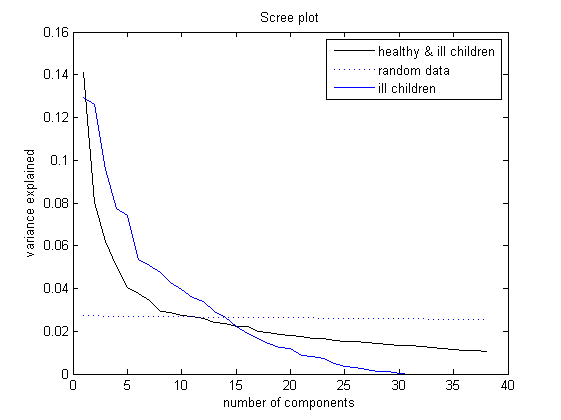
\includegraphics[scale=0.95]{img/pca_scree.png}
\end{figure}

In the illustration, we can see that the first component explains 14.12\% of the variance in the data, and that in order to explain more than 65\% (65.54\%), 15 out of the 38 components are needed.  Also, it seems that the variance within the \textit{ill} examples can be captured in a better way: the first component only explains 12.93\% of the variance in the data, but 65.52\% of the variance can be captured by 'only' 8 components.
The scree plot clearly shows that compression of the data is very costly, which means that most of the original features do not contain a lot of information (but clearly more than random data).

When we only keep the two most informative principal components, we can plot the resulting (transformed) dataset in a 2D-plot. The following illustration shows the resulting visualisation, where the positive (\textit{ill}) and negative (\textit{healthy}) examples are marked with different symbols. Although the plot suggests the presence of some clusters within the data, it is clear that the positive examples are scattered completely amongst the distribution of the negative examples and that no clear separation exists at this level.

\begin{figure}[h]
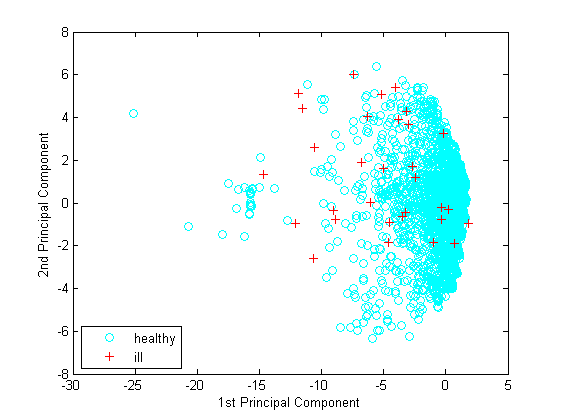
\includegraphics[scale=0.95]{img/pca_space.png}
\end{figure}


Another approach to analyse the data, is to find out how close features are related to each other. This can for example be achieved with \textbf{Multidimensional Scaling} (MDS), another linear technique with a similar aim as PCA.  MDS finds a low-dimensional projection of the data such as to preserve, as closely as possible, the pairwise distances between data points.  In the case where the distances are Euclidian, it gives equivalent results to PCA~\cite{bishop}.
We can obtain a distance matrix of the dataset by calculating its correlation matrix and transforming it such that the elements represent dissimilarities (in stead of similarities). When we perform MDS on this matrix, we can plot the (dis)similarities between all the features in a 2D-plot.\\
The following illustration shows the (dis)similarities between the features of the \textit{ill children} dataset after performing MDS. The features are labeled by an ID explained earlier in~\ref{ill-coding}.


\newpage

%\begin{landscape}
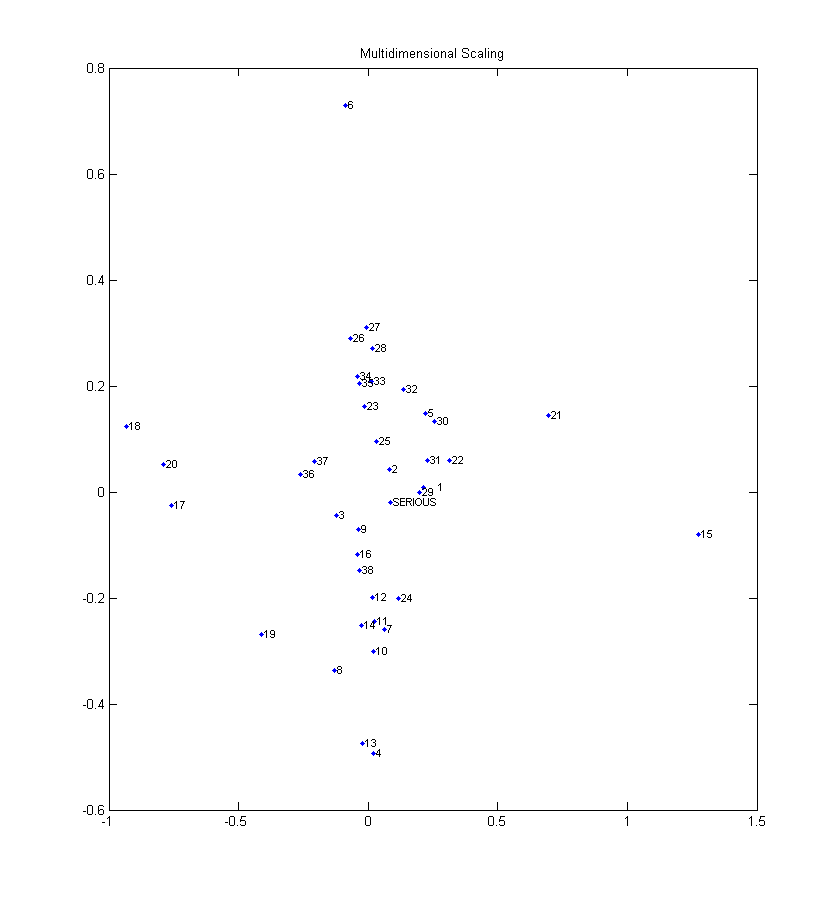
\includegraphics[scale=0.70]{img/mds_corr_stdN.png}
%\end{landscape}

Summarized, we can say that the data does not contain a high degree of correlated features, and that there exists no clear separation of the positive instances. Since the minority data is moreover described by more dimensions than it is populated by examples, we can expect difficulties when modeling the data distribution for sampling purposes. Important features regarding the final outcome seem to be: tachypnoea, age, gender, the total duration of the illness, unconsciousness, headache, Something Wrong, breathing problems, crepetitations and incoherentness. Less important features are: temperature, Urinary Tract Infection, diarrhoea, tummyache, vomiting, and cough.


%-------------------------------------------------------------------------------------------------------------------
% THE CLASSIFIERS
%-------------------------------------------------------------------------------------------------------------------
\newpage
\section{Learning Algorithms}\label{theclassifiers}
In this section we give a brief overview of the learning algorithms that are used in the experiments. With the exception of CART, these algorithms are provided by Weka, a Java Opensource (GNU General Public License) software collection of machine learning algorithms for data mining tasks (\url{http://www.cs.waikato.ac.nz/ml/weka}). The experiments of CART are performed with \textit{rpart} (\url{http://cran.r-project.org/web/packages/rpart/}).

\subsection{J48}
J48 is a learning algorithm for generating a pruned or unpruned C4.5 decision tree~\cite{J48}. The main approach of these classifiers was discussed in section~\ref{classifier-example}. Additionally to explained capabilities, J48 is able to evaluate continuous features and to handle missing feature values. An important modeling choice in this learning algorithm regards the \textit{confidence factor}, which is used for pruning (smaller values incur more pruning).

\subsection{JRip}
JRip is an implementation of Repeated Incremental Pruning to Produce Error Reduction (RIPPER), an optimized version of the propositional rule learner IREP. The learning algorithm consists of three stages. In the first stage, rules are growed and pruned using the concept of information gain. In the second stage, generated rules are examined and optimized for generalization purpose (using the concept of Description Length). Finally, rules that hinder generalisation are deleted in the third stage. An important modeling choice in J48 defines whether decision rules are pruned or not.~\cite{jrip}

\subsection{Naive Bayes}
The Naive Bayes algorithm is a learning algorithm based on Bayes rule, that assumes the features $X_1 \ldots X_m$ are all conditionally independent of one another, given $Y$. The value of this assumption is that it dramatically simplifies the representation of $P(x|y)$, and the problem of estimating it from the training data. In order to deal with continuous features, two approaches are suggested. The first approach involves density estimation by a Gaussian distribution. The second approach involves density estimation by a nonparametric kernel~\cite{John95estimatingcontinuous}. Naive Bayes learning turns out to do surprisingly well in a general-purpose learning algorithms; the boosted version is one of the most effective general-purpose learning algorithms.  Naive Bayes scales well to very large problems: with $n$ Boolean features, there are just \(2n+1\) parameters to estimate, and no search is required to find the maximum-likelihood Naive Bayes hypothesis.  Finally, Naive Bayes learning has no difficulty with noisy data and can give probabilistic predictions when appropriate~\cite{Russell07Artificial}.

\subsection{IBk}
IBk is Weka's implementation for K-nearest neighbor learning (kNN), one of the most basic lazy (or: instance-
based) learning methods. This means that it does not explicitly induce a representation of the target function, but rather stores the training data during the training phase. More specifically, kNN simply retrieves the \(k\) nearest neighbors of a presented instance from training data, and classifies that instance according to a voting scheme that is applied to the classes of these neighbors. Generalisation beyond training data is achieved  according to the assumption that the classification of a query instance should be oriented on those instances which are nearby in feature space. The parameter \(k\) is a direct lever for adjusting the degree of fit to the training data. As a result, nearest neigbhour (NN) learning algorithms have several benefits:

\begin{itemize}
\item simple representations for concept descriptions
\item low incremental learning costs
\item small storage requirements
\item ability to produce concept exemplars on demand
\item ability to learn continuous functions
\item ability to learn non-linearly separable categories
\end{itemize}

An important backdraw of NN learning algorithms is the fact that they are highly sensitive to noise. For this purpose, an extension has been introduced by Aha \& Kibler, which identifies and eliminates noisy concept description instances~\cite{Aha91instance-basedlearning}.

\subsection{SMO}
Sequential Minimal Optimization (SMO) was introduced by John Platt's~\cite{Platt98machines} in order to train a support vector machine (SVM). SVMs are based on the concept of decision planes that define decision boundaries. In order to allow complex decision boundaries, training instances are rearranged using a set of mathematical functions (kernels) such that they become linearly separable. This mapping technique however implies a complex optimization problem, also known as the quadratic programming (QP) optimization.  SMO breaks this problem into a series of smallest possible QP problems, which are then solved analytically. This avoids using a time-consuming numerical QP optimization as an inner loop. Because matrix computation is avoided, SMO scales somewhere between linear and quadratic in the training set size for various test problems, while the standard chunking SVM algorithm scales somewhere between linear and cubic in the training set size~\cite{Platt98smo}. Weka's implementation normalizes all features by default, globally replaces all missing values and transforms nominal attributes into binary ones.

\subsection{CART}
Classification and Regression Tree analysis (CART)~\cite{Bk1871082462} involves using binary trees for tackling classification and regression problems. Basically, the algorithm calculates at each node of the decision tree which variable is the \textit{most discriminating} (using the Gini index) and constructs at that node a bifurcation of two branches. Instead of employing stopping rules, CART generates a sequence of subtrees by growing a large tree and pruning it back until only the root node is left. Then it uses cross-validation to estimate the misclassification cost of each subtree and chooses the one with the lowest estimated cost. As a result, since multiple trees must be built and pruned, the procedure used for pruning is more complex (and therefore more time consuming) than C4.5's pruning, but tends to produce smaller trees~\cite{oatesJensen97}. This technique has a number of advantages over other classification methods, including multivariable logistic regression. First, it is inherently non-parametric, meaning no assumptions have to be made about the underlying distribution. Secondly, the resulting classifiers summarized in a tree are simpler to interpret than multivariable logistic regression classifiers, making it more practical in a clinical setting. However, it should be noted that CART also has some undesirable properties~\cite{cartLoh}: first, the splitting method is biased towards variables that have more distinct values. Sencondly, the exponential number of splits for categorical variables causes serious computational difficulties when the number of distinct values a variable can take is large and \textit{y} takes more than two values. Finally, the algorithm is also biased towards variables with more missing values.

%-------------------------------------------------------------------------------------------------------------------
% Experiments on existing approaches
%-------------------------------------------------------------------------------------------------------------------
\section{Experiment results of discussed approaches}\label{compex}
In this section, we present the experiment results of discussed approaches in chapter~\ref{imbalanced}, applied on the dataset of KULeuven. We evaluate the classifiers by applying stratified 10-fold cross-validation (which is repeated over 10 randomized runs) and measuring the AUC, sensitivity and specificity. A summary of these experiments can be found in section~\ref{exp-summary}.
%-------------------------------------------------------------------------------------------------------------------
% Cost-sensitivity
%-------------------------------------------------------------------------------------------------------------------
\subsection{Cost-Sensitive Learning}\label{costsensitive}
In this section, we investigate the effect of introducing cost-sensitivity in the discussed classifiers. Cost-sensitivity is obtained by reweighting training instances according to a certain sample ratio (as discussed in section~\ref{cost-sensitivity}). In these experiments, the cost of misclassifying minority instances is gradually increased as such that higher sensitivities can be obtained. In order to have a better view into the effect of increasing costs, misclassification costs are often log-plotted (\textit{log10}). Since Weka does not support CART, another software package (\textit{rpart} - \url{http://cran.r-project.org/web/packages/rpart/}) was used to analyse this learning algorithm. This package allows incorporation of variable and possibly non-symmetric misclassification costs into the splitting rule via prior specification. It should however be noted that \textit{rpart} does not provide cross-validation support for evaluating the actual classifier prediction power (which is not to be confused with the internally used cross-validation in order for classifier selection).


\newpage
\begin{figure}[h]
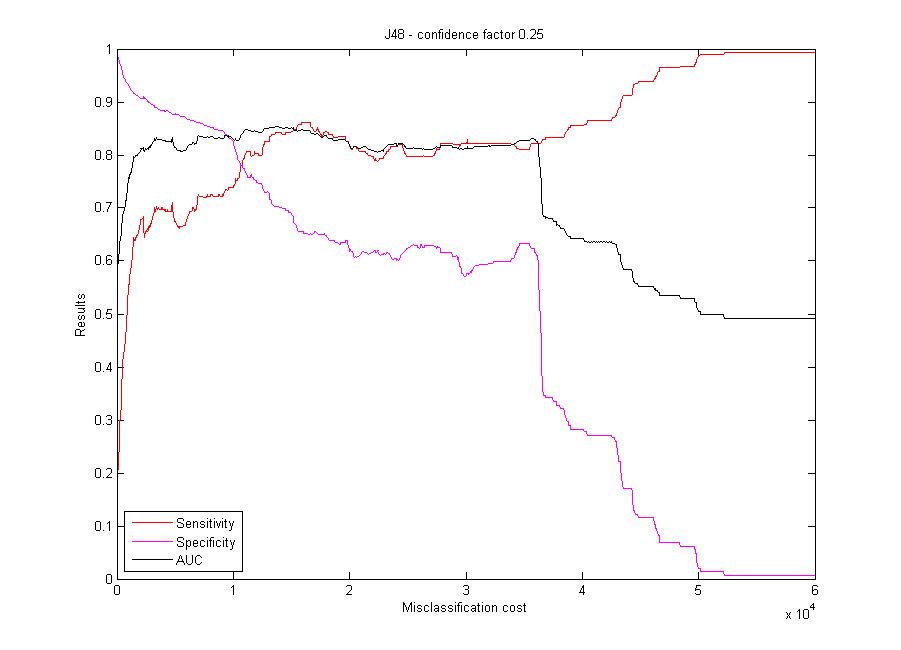
\includegraphics[scale=0.65]{img/J48-confid025.png}
\caption{\textbf{Cost-sensitivity and J48} (confidence factor 0.25) - The classifier resulting into the highest AUC (0.8536) is obtained with a misclassification cost of 13\,250 and yields a sensitiviy of 83.87\% and specificity of 71.44\%. At a misclassification cost of around 36000, a significant drop in specificity and AUC occurs against only a very small increase in sensitivity.}
\end{figure}

\newpage
\begin{figure}[h]
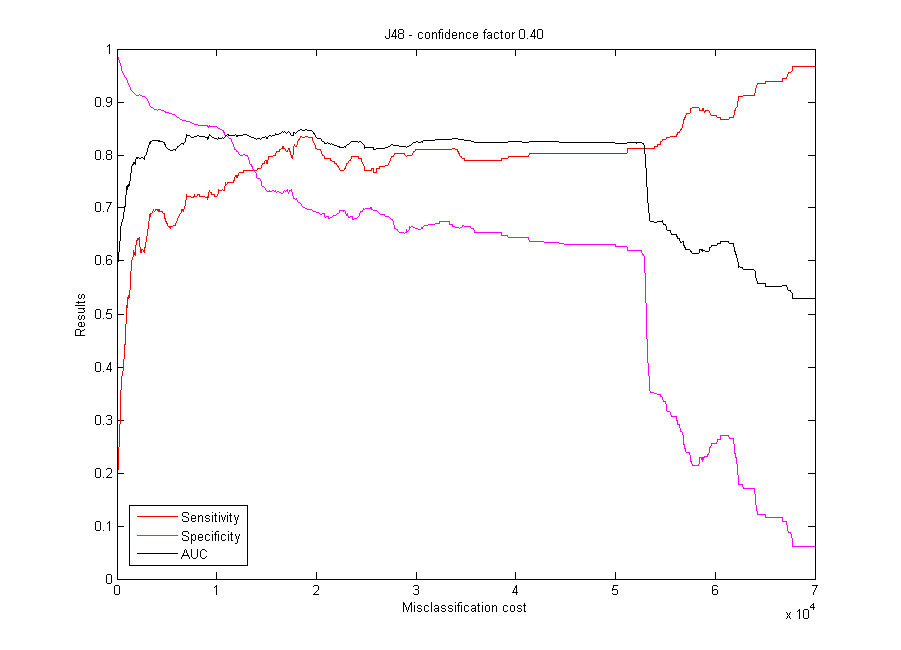
\includegraphics[scale=0.65]{img/J48-confid040.png}
\caption{\textbf{Cost-sensitivity and J48} (confidence factor 0.40) - The classifier resulting into the hightest AUC (0.8487) is obtained with a misclassification cost of 18\,400 and yields a sensitivity of 83.55\% and specificity of 70.81\%.  Again, a significant drop in specificity and AUC against a small increase in sensitivity occurs around a misclassification cost of 53000.}
\end{figure}

\newpage
\begin{figure}[h]
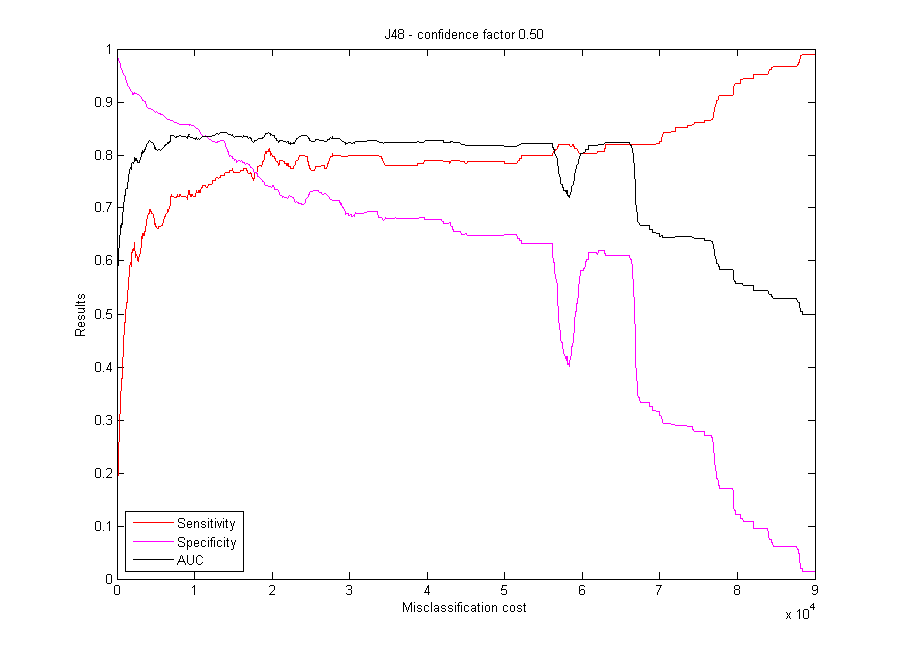
\includegraphics[scale=0.65]{img/J48-confid050.png}
\caption{\textbf{Cost-sensitivity and J48} (confidence factor 0.65) - The classifier resulting into the hightest AUC (0.8431) is obtained with a misclassification cost of 19\,600 and yields a sensitivity of 81.29\% and specificity of 73.93\%.  Two times, a significant drop in specificity occurs which is only recovered once.}
\end{figure}

\newpage
\begin{figure}[h]
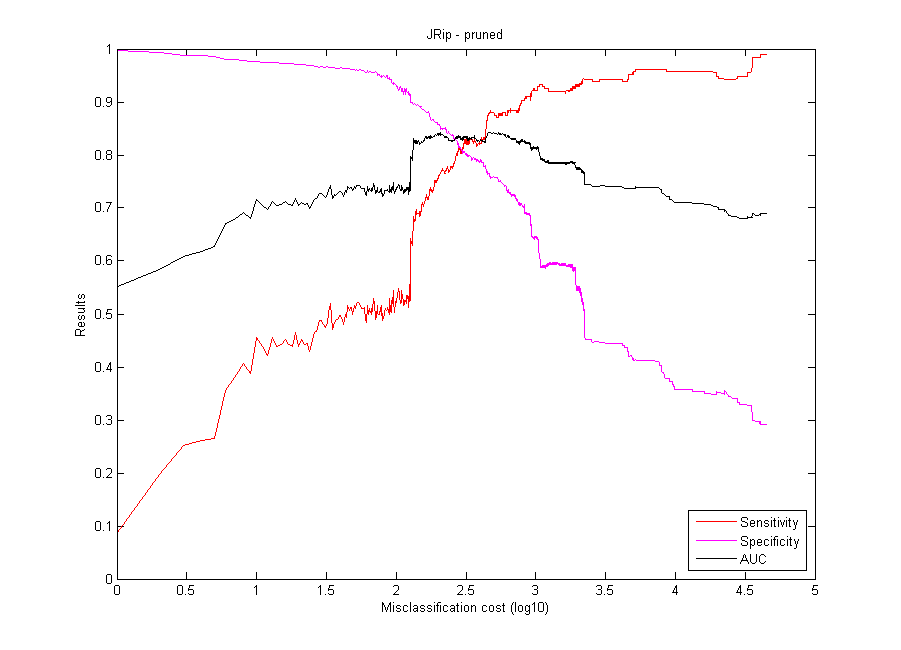
\includegraphics[scale=0.65]{img/jrip.png}
\caption{\textbf{Cost-sensitivity and JRip} (pruned decision rules) - JRip appears to achieve quite fast high sensitivities: at a misclassification cost of 466, a sensitivity of 87.74\% and specificity of 76.50\% is obtained (AUC: 0.8431). Obtaining higher sensitivities however becomes very costly: a sensitivity of 90.32\% is reached at a cost of 787 (specificity: 70.57\%), a higher sensitivity of 94.19\% at cost 2160 (specificity: 51.81\%). To achieve a 99.03\% sensitivity rate, costs have to be increased up to  40\,890, leaving a specificity of only 29.13\%.}
\end{figure}

\newpage
\begin{figure}[h]
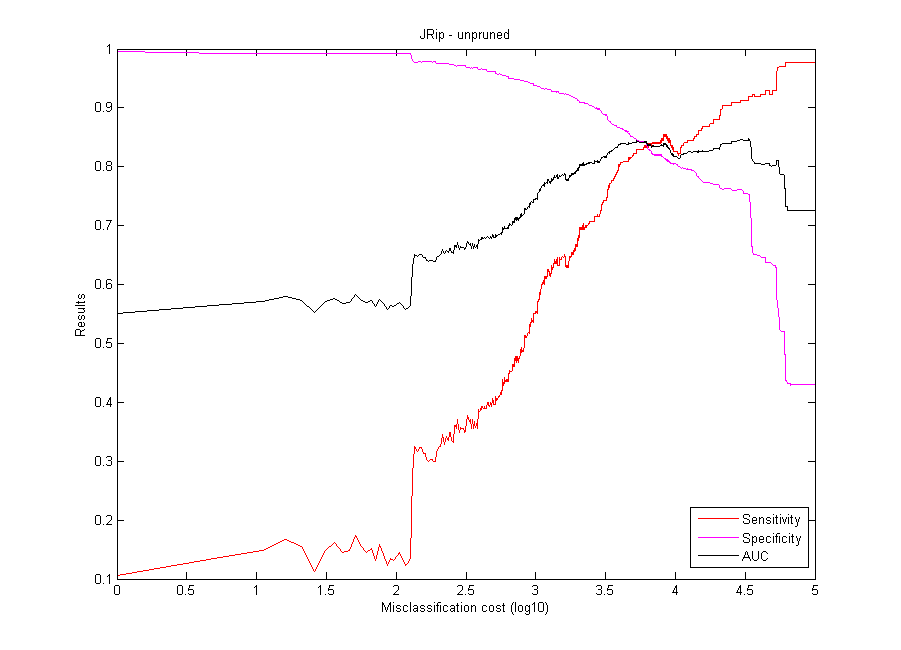
\includegraphics[scale=0.65]{img/jrip-nopruning.png}
\caption{\textbf{Cost-sensitivity and JRip} (unpruned decision rules) - Unpruned decision rules appear to have a positive effect on the sensitivities: at a misclassification cost of 33350, a sensitivity of 91.94\% and specificity of 75.33\% is obtained (AUC: 0.8473). Obtaining higher sensitivities however  becomes very costly: a sensitivity of 94.84\% is reached at a cost of 52985 (specificity: 60.90\%).}
\end{figure}

\newpage
\begin{figure}[h]
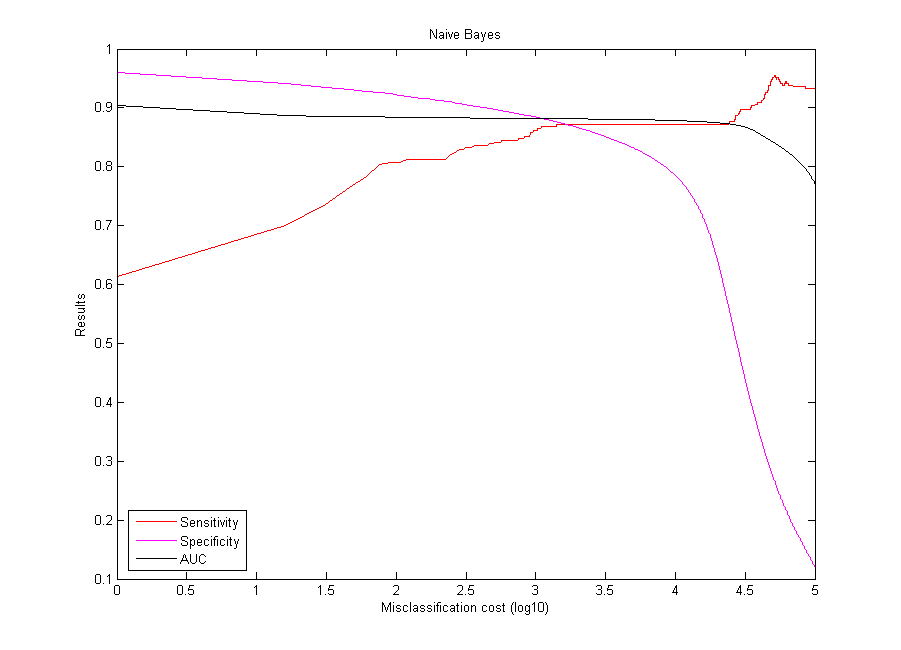
\includegraphics[scale=0.65]{img/naivebayes.png}
\caption{\textbf{Cost-sensitivity and Naive Bayes} (Laplace smoothing) - Experiment results of cost-sensitive learning with Naive Bayes using the Laplace estimate.}
\end{figure}

\newpage
\begin{figure}[h]
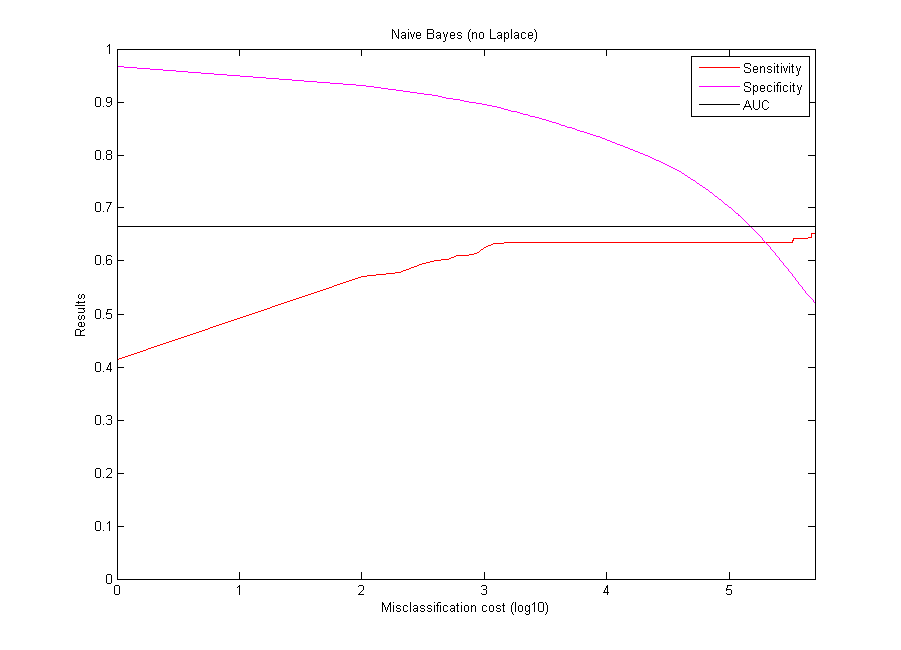
\includegraphics[scale=0.65]{img/naivebayes-nolaplace.png}
\caption{\textbf{Cost-sensitivity and Naive Bayes} (no smoothing) - Experiment results of cost-sensitive learning with Naive Bayes using no smoothing estimate.}
\end{figure}

\newpage
\begin{figure}[h]
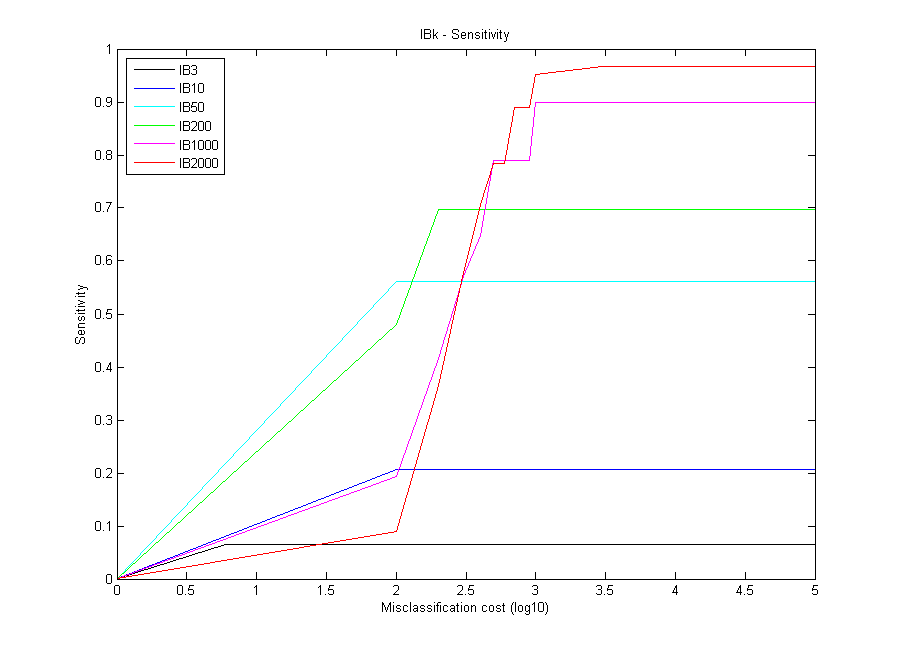
\includegraphics[scale=0.65]{img/IBk_sens.png}
\caption{\textbf{Cost-sensitivity and IBk} (Sensitivities) - Sensitivities mainly seems to be affected by the number of evaluated nearest neighbours, rather than the applied misclassification cost. Although the positive instance weight influences the sensitivity in an early stage, further increase does not lead to any improvements unless the number of nearest neighbours is increased. IB3 reaches a maximum sensitivity of 6.45\%, IB10 20.65\%, IB50 56.13\%, IB200 69.68\%, IB1000 90\% and IB2000 96.77\%.}
\end{figure}

\newpage
\begin{figure}[h]
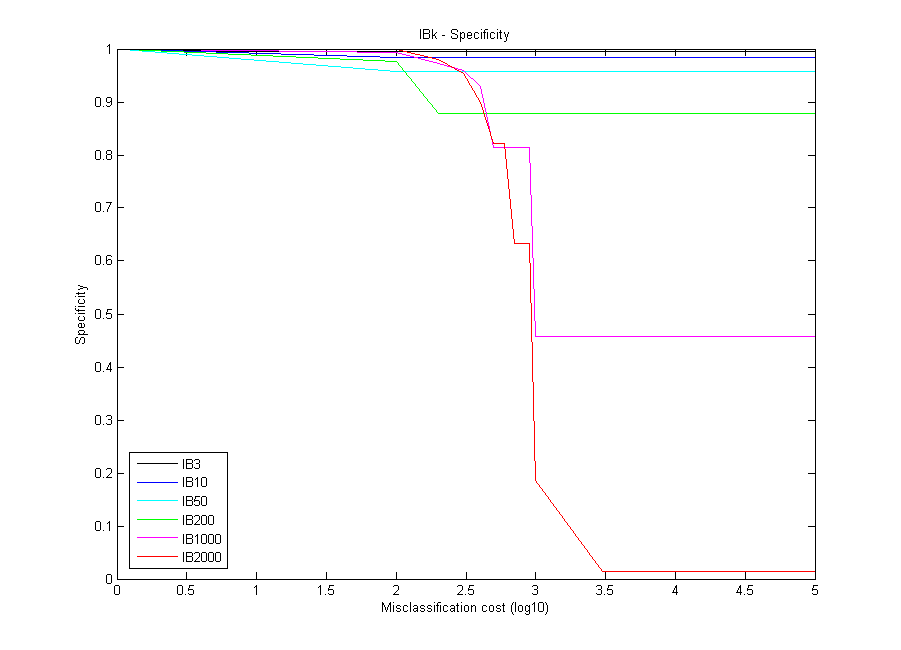
\includegraphics[scale=0.65]{img/IBk_spec.png}
\caption{\textbf{Cost-sensitivity and IBk} (Specificities) - A similar situation as in the sensitivities occurs with the specificities. Once the highest sensitivity is reached, specificities remain steady unless the number of nearest neighbours is increased. At the highest sensitivity of IB3, a specificity of 99.59\% holds, for IB10 98.48\%, for IB50 95.71\%, for IB200 87.77\%, for IB1000 45.66\% and for IB2000 1.48\%.}
\end{figure}

\newpage
\begin{figure}[h]
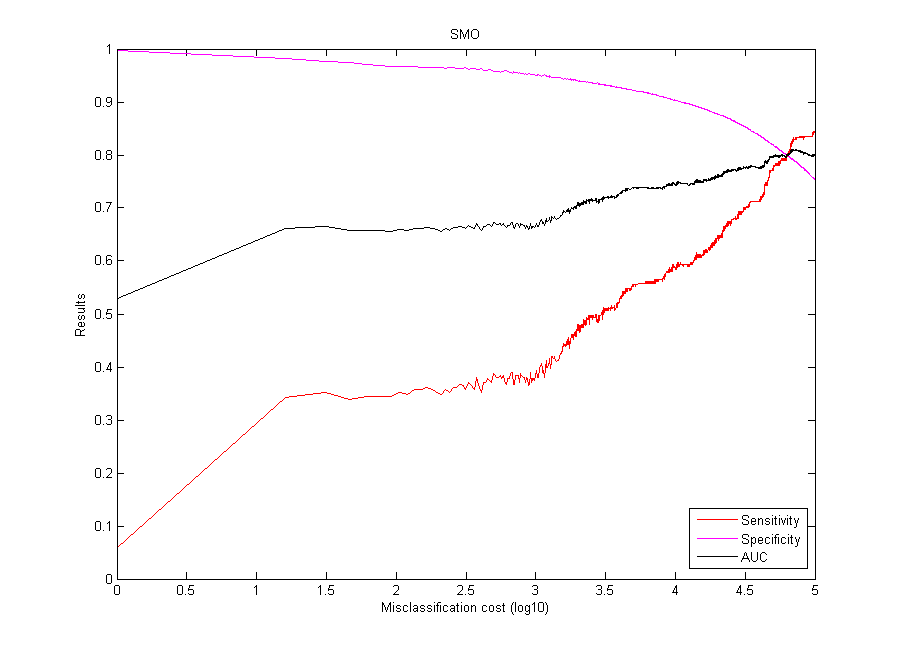
\includegraphics[scale=0.65]{img/smo.png}
\caption{\textbf{Cost-sensitivity and SMO} (complexity parameter $c=1$, linear exponent) - Experiment results of cost-sensitive learning with SMO.}
\end{figure}

\newpage
\begin{figure}[h]
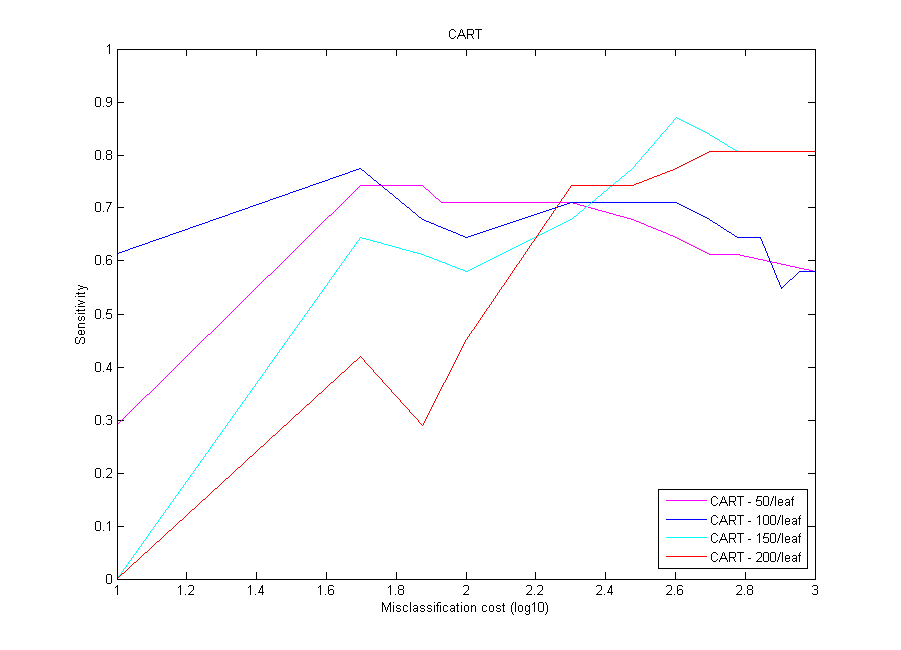
\includegraphics[scale=0.65]{img/CART_sens.png}
\caption{\textbf{Cost-sensitivity and CART}  (Sensitivities) - In this experiment, 4 different types of classifiers were built using a different minimum number of observations (50, 100, 150 and 200) that must exist in a node or a terminal node . Results show that how lower the minimum number of observations in a node or terminal node becomes, how lower the sensitivities become (although the perfomance on the training set increases). }
\end{figure}

\newpage



\begin{figure}[h]
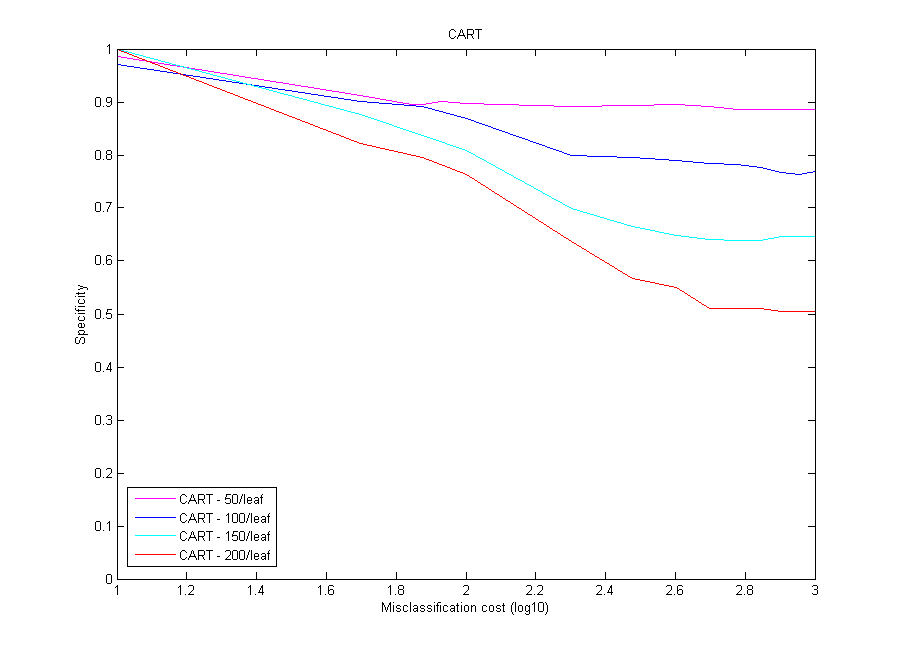
\includegraphics[scale=0.65]{img/CART_spec.png}
\caption{\textbf{Cost-sensitivity and CART} (Specificities) - In the specificities, the cost increase yields less performance degrade when the minimum number of observations in a (terminal) node is low.}
\end{figure}


%-------------------------------------------------------------------------------------------------------------------
% MetaCost
%-------------------------------------------------------------------------------------------------------------------
\newpage
\subsection{MetaCost}\label{exp-metacost}
In this section, we introduce cost-sensitivity by applying MetaCost on the discussed classifiers. In order to keep the number of experiments realistic, we only test those types of classifiers that proved most promising (highest AUC) in cost-sensitivity analysis.  

\begin{figure}[h]
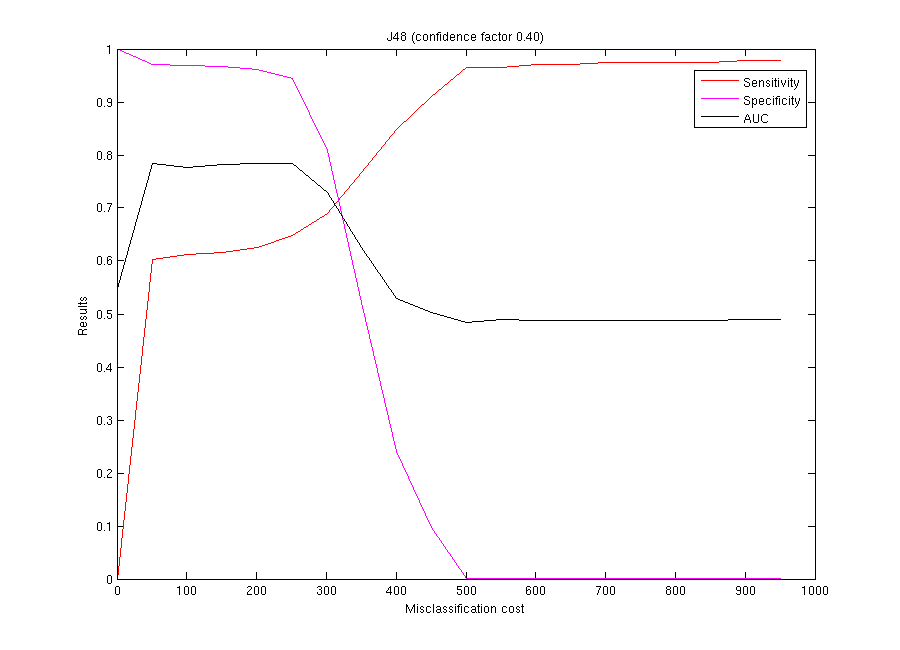
\includegraphics[scale=0.65]{img/MC_J48-confid040.png}
\caption{\textbf{MetaCost with J48} (confidence factor 0.65) - Experiment results of MetaCost with J48. MetaCost allows J48 to achieve a maximum AUC of 0.7846 at a misclassification cost of 251. This classifier yields a sensitivity of 64.84\% and a specificity of 94.51\%. A sensitivity of 90.97\% is achieved using a misclassification cost of 451, and yields a specificity of 9.71\%. Finally, a maximum sensitivity of 97.74\% is obtained together with a specificity of 0.00\%.}
\end{figure}

\newpage
\begin{figure}[h]
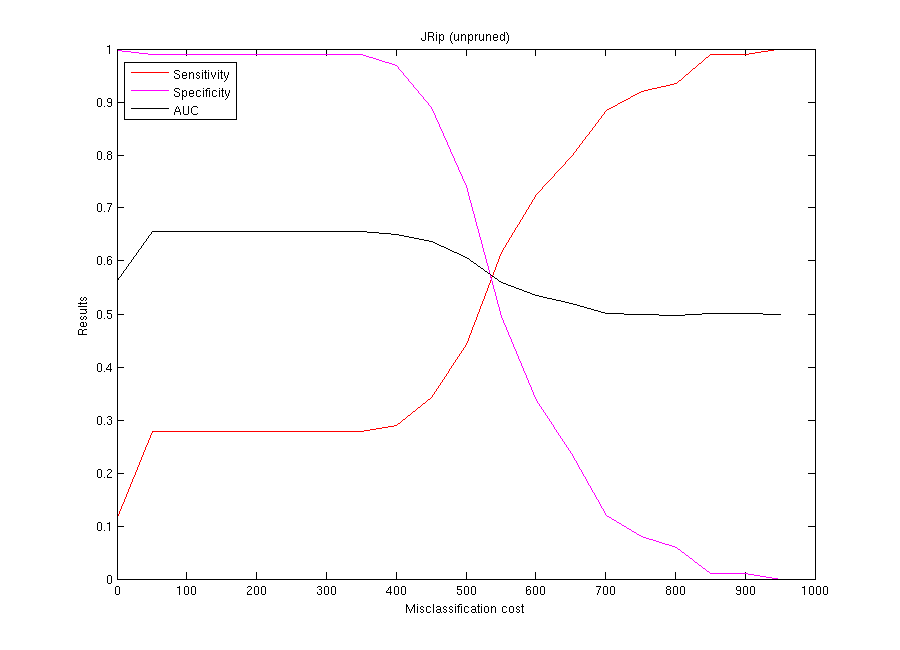
\includegraphics[scale=0.65]{img/MC_JRip-unpruned.png}
\caption{\textbf{MetaCost with JRip} (unpruned decision rules) - Experiment results of MetaCost with JRip. MetaCost allows JRip to achieve a maximum AUC of 0.6565 at a misclassification cost of 51. This classifier yields a sensitivity of 27.74\% and a specificity of 98.87\%. A sensitivity of 91.94\% is achieved using a misclassification cost of 751, and yields a specificity of 7.93\%. Finally, a maximum sensitivity of 100.00\% is obtained together with a specificity of 12.54\%.}
\end{figure}

\newpage
\begin{figure}[h]
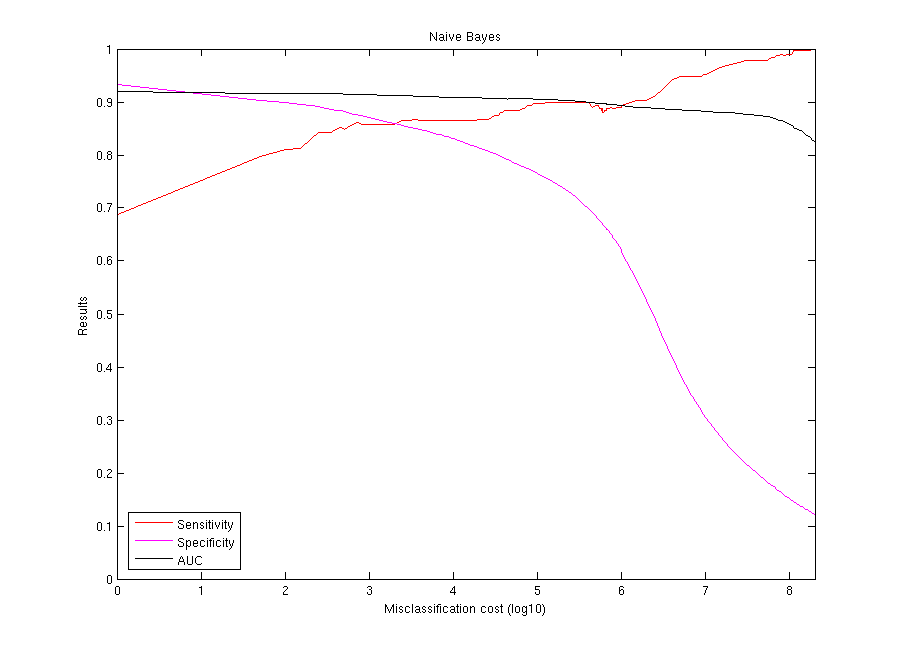
\includegraphics[scale=0.65]{img/MC_Naivebayes.png}
\caption{\textbf{MetaCost with Naive Bayes} (Laplace smoothing) - MetaCost allows Naive Bayes to achieve a maximum AUC of 0.9206 at a misclassification cost of 1. This classifier yields a sensitivity of 68.71\% and a specificity of 93.28\%. A sensitivity of 90.32\% is achieved using a misclassification cost of 1\,500\,000, and yields a specificity of 56.53\%. Finally, a maximum sensitivity of 100.00\% is obtained together with a specificity of 0.00\%.}
\end{figure}

\newpage
\begin{figure}[h]
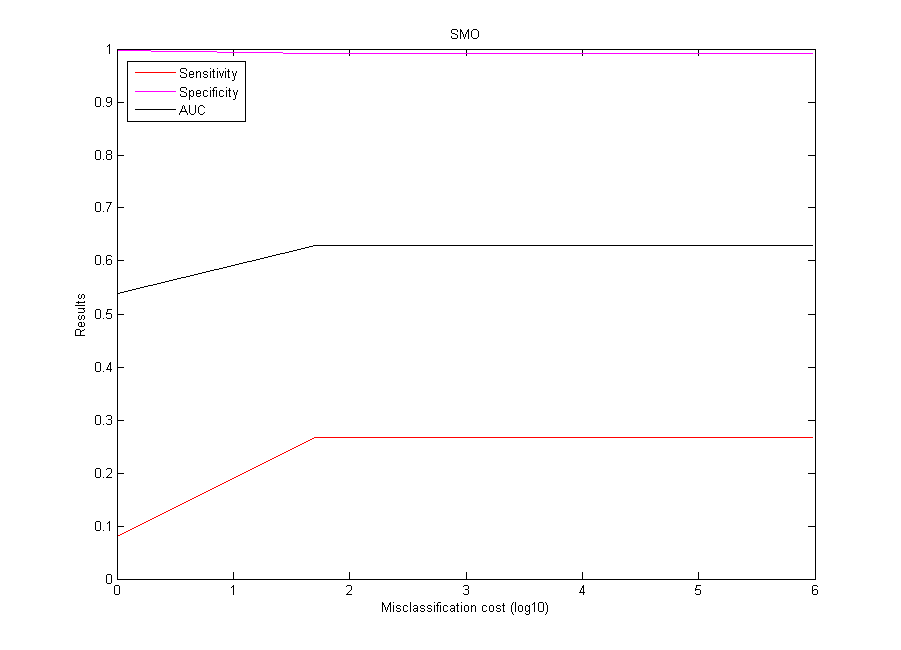
\includegraphics[scale=0.65]{img/MC_SMO.png}
\caption{\textbf{MetaCost with SMO} - MetaCost allows SMO to achieve a maximum AUC of 0.6299 at a misclassification cost of 51. This classifier yields a sensitivity of 26.77\% and a specificity of 99.22\%. When costs are further increased up to 1\,000\,000, no different models are obtained.}
\end{figure}


%-------------------------------------------------------------------------------------------------------------------
% SMOTE
%-------------------------------------------------------------------------------------------------------------------
\newpage
\subsection{SMOTE}\label{exp-SMOTE}
In this section, we apply the Synthetic Minority Over-sampling Technique (SMOTE) using 5 nearest neighbours. In order to keep the number of experiments realistic, we only test those types of classifiers that proved most promising (highest AUC) in cost-sensitivity analysis.

\begin{figure}[h]
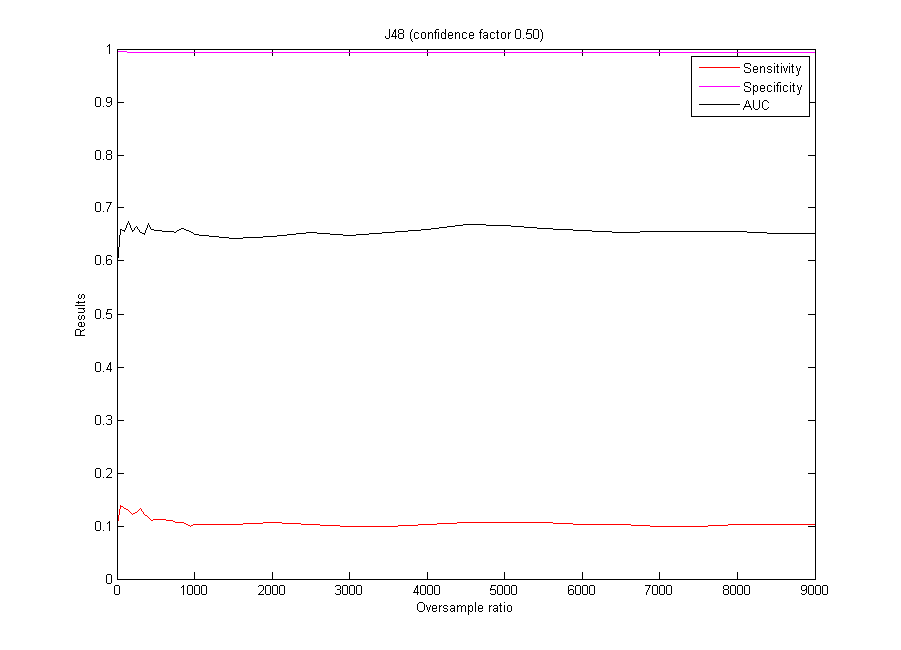
\includegraphics[scale=0.65]{img/SMOTE_J48-confid-050.png}
\caption{\textbf{SMOTE and J48} (confidence factor 0.50) - The generation of synthetic instances seems to have rather a limited/negative effect in favouring the recognition rate of the minority samples. A maximum AUC of 0.6750 is achieved at a  misclassification cost of 150. This classifier yields a sensitivity of 12.90\% and a specificity of 99.33\%. At a misclassification cost of 51, a maximum sensitivity of 13.87\% is obtained (specificity: 99.55\%).
}
\label{fig:exp-smote-j48}
\end{figure}

\newpage
\begin{figure}[h]
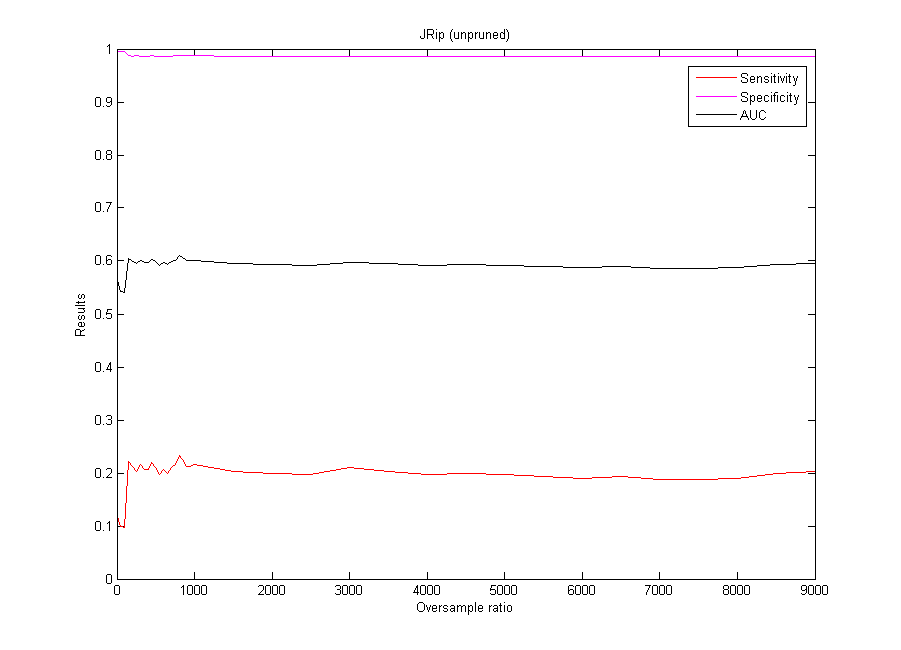
\includegraphics[scale=0.65]{img/SMOTE_JRip-unpruned.png}
\caption{\textbf{SMOTE and JRip} (unpruned decision rules) - A similar sitation as in~\ref{fig:exp-smote-j48} occurs, however a higher sensitivity is obtained. A maximum AUC of 0.6096 is achieved at a misclassification cost of 800. This classifier also yields the maximum sensitivity of 23.23\% (specificity: 98.70\%).}
\end{figure}

\newpage
\label{exp-smote-nb}
\begin{figure}[h]
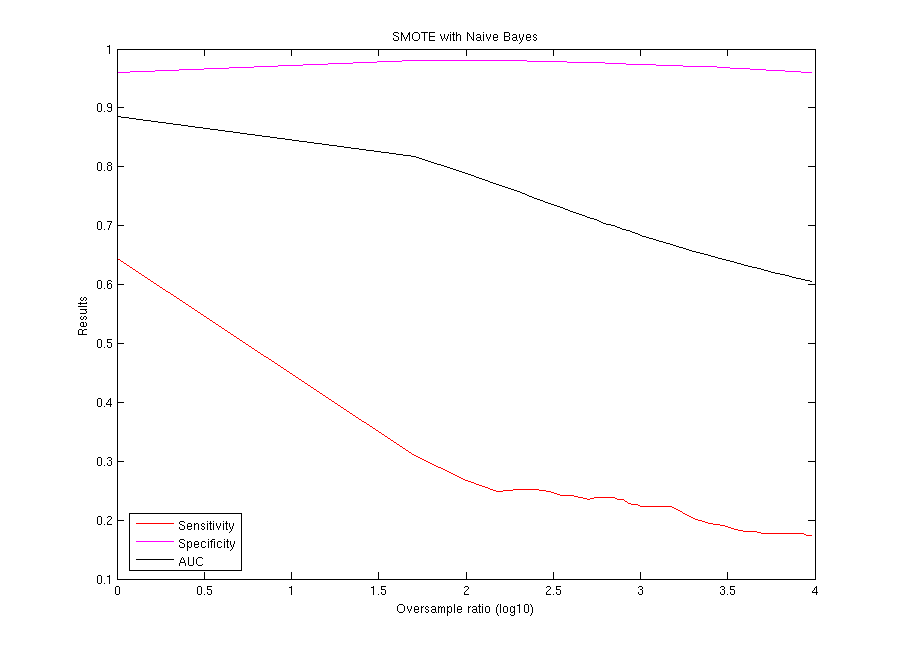
\includegraphics[scale=0.65]{img/smote.png}
\caption{\textbf{SMOTE and Naive Bayes} (Laplace smoothing) - applying SMOTE clearly worsens the performance with a Naive Bayes classifier.  A maximum AUC of 0.8851 is achieved at a  misclassification cost of 1. This classifier also yields the maximum sensitivity of 64.51\% (specificity: 95.94\%).}
\end{figure}

\newpage
\begin{figure}[h]
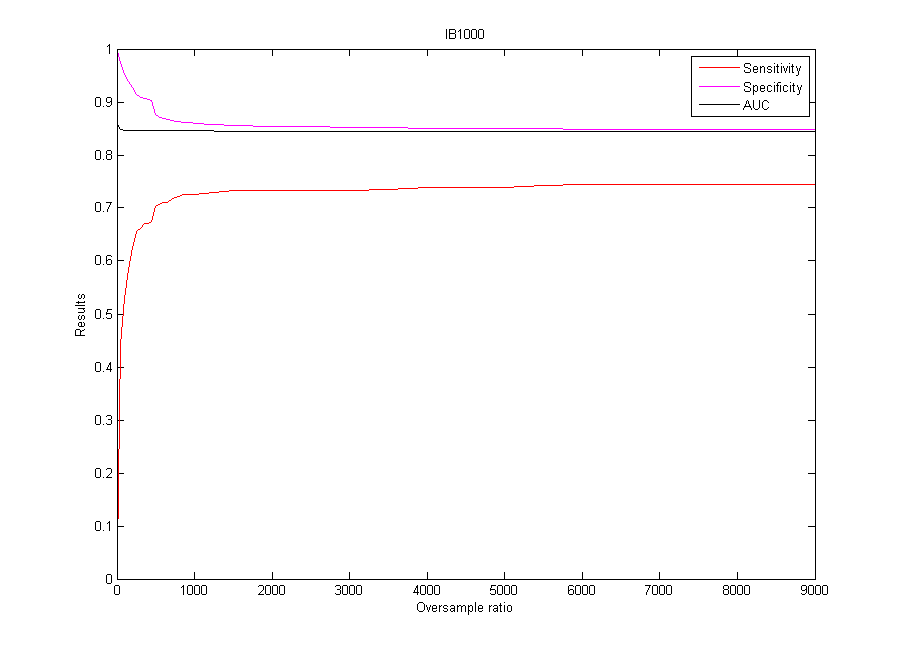
\includegraphics[scale=0.65]{img/SMOTE_IB1000.png}
\caption{\textbf{SMOTE and IBk} (1000NN) - IBk is the only classifier SMOTE seems to perform well with. A maximum AUC of 0.8616 is achieved at a  misclassification cost of 1. This classifier yields a sensitivity of 0.00\% and a specificity of 100.00\%. At a misclassification cost of 6000, a maximum sensitivity of 74.52\% is obtained (specificity: 84.88\%).}
\end{figure}

\newpage
\begin{figure}[h]
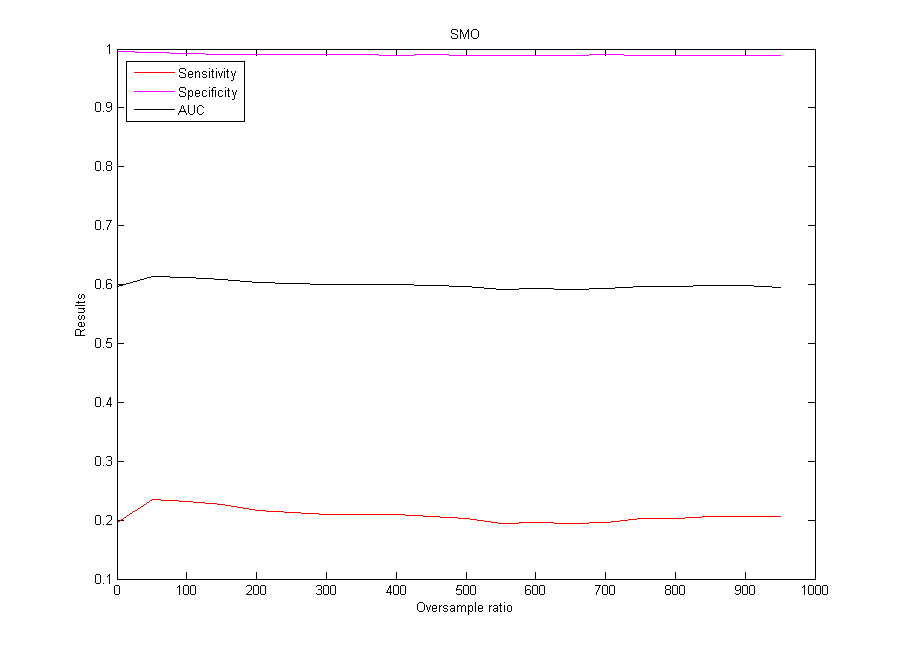
\includegraphics[scale=0.65]{img/SMOTE_SMO.png}
\caption{\textbf{SMOTE and SMO} (complexity parameter $c = 1$, linear exponent) - Experiment results of SMOTE with SMO. A maximum AUC of 0.6145 is achieved at a  misclassification cost of 50. This classifier also yields a maximum sensitivity of 23.55\% (specificity: 99.35\%).}
\end{figure}

%-------------------------------------------------------------------------------------------------------------------
% Bagging
%-------------------------------------------------------------------------------------------------------------------
\newpage
\subsection{Bagging for Imbalanced Datasets}\label{exp-bagging}
Bagging for Imbalanced Data is an extension to regular bagging which was proposed by Tao et al.~\cite{1137548}. The approach consists of generating bootstrap samples where the several classes are sampled with different ratios, hence achieving over- and/or under-sampling. In the following experiments, we create an ensemble of 10 classifiers which are trained on bootstraps where the minority class is over-sampled. In order to keep the number of experiments realistic, we only test those types of classifiers that proved most promising (highest AUC) in cost-sensitivity analysis.

\begin{figure}[h]
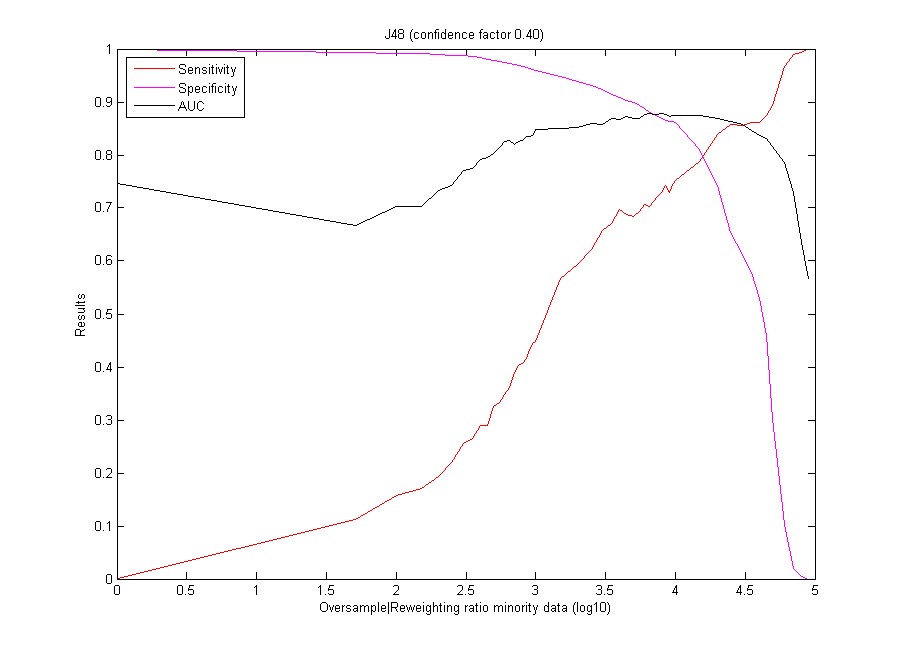
\includegraphics[scale=0.65]{img/bi_J48-confid040.png}
\caption{\textbf{Bagging with J48} (confidence factor 0.40) - Experiment results of Bagging for Imbalanced Datasets with J48. This technique allows J48 to achieve a maximum AUC of 0.8783 at a misclassification cost of 6\,500. This classifier yields a sensitivity of 70.32\% and a specificity of 88.06\%. A sensitivity of 96.77\% is achieved using a misclassification cost of 60\,000, and yields a specificity of 10.36\%. Finally, a maximum sensitivity of 100.00\% is obtained together with a specificity of 0.00\%.}
\end{figure}

\newpage
\begin{figure}[h]
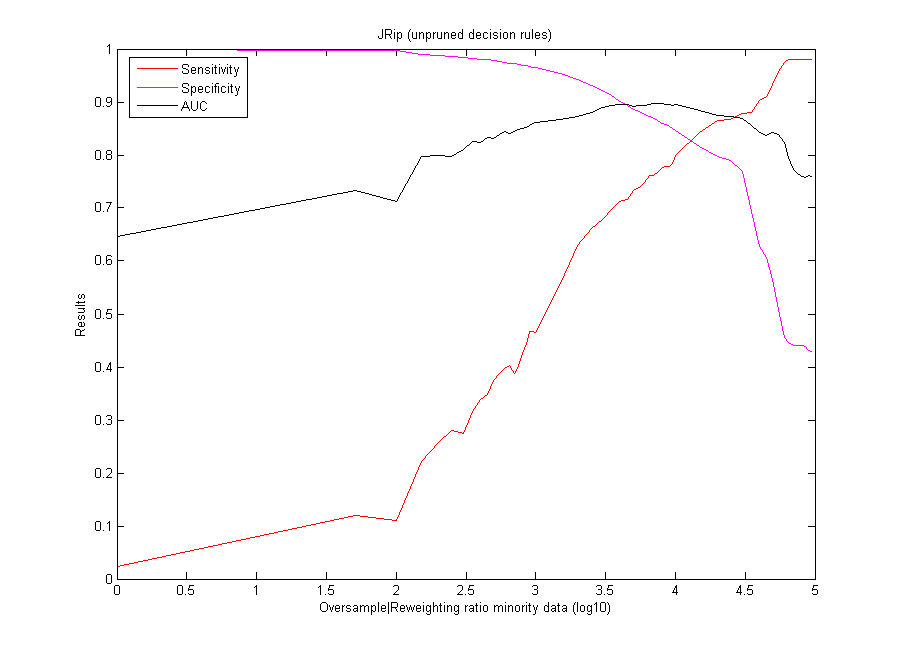
\includegraphics[scale=0.65]{img/bi_JRip-unpruned.png}
\caption{\textbf{Bagging with JRip} (unpruned decision rules) - Experiment results of Bagging for Imbalanced Datasets with JRip. This technique allows JRip to achieve a maximum AUC of 0.8976 at a misclassification cost of 7\,001. This classifier yields a sensitivity of 76.13\% and a specificity of 86.82\%. A sensitivity of 90.32\% is achieved using a misclassification cost of 40\,001, and yields a specificity of 62.80\%. Finally, a maximum sensitivity of 98.06\% is obtained together with a specificity of 44.56\%.}
\end{figure}

\newpage
\begin{figure}[h]
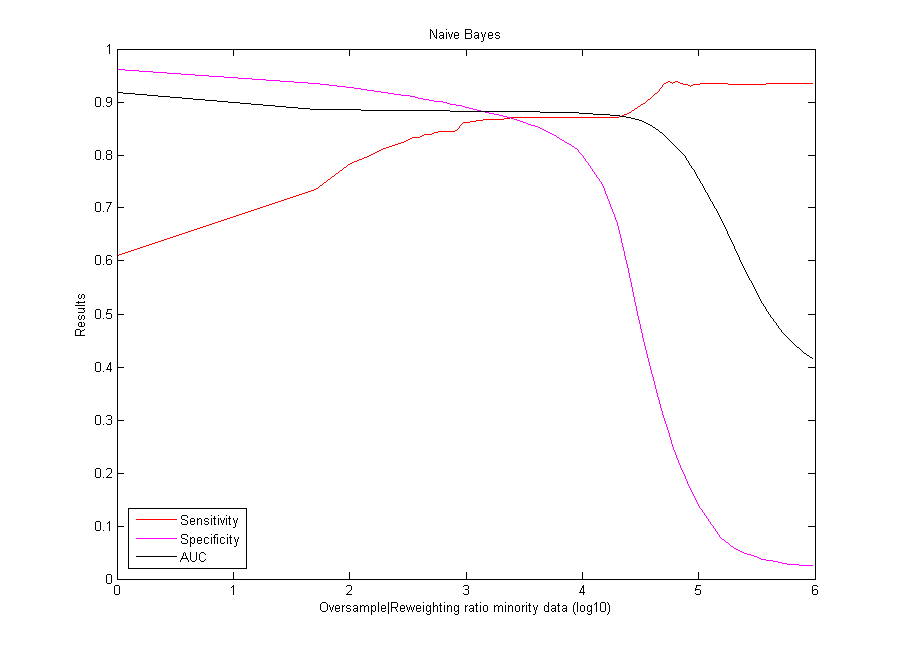
\includegraphics[scale=0.65]{img/bi_NaiveBayes.png}
\caption{\textbf{Bagging with Naive Bayes} - Experiment results of Bagging for Imbalanced Datasets with Naive Bayes. This technique allows Naive Bayes to achieve a maximum AUC of 0.9180 at a misclassification cost of 1. This classifier yields a sensitivity of 60.97\% and a specificity of 96.16\%. A sensitivity of 90.32\% is achieved using a misclassification cost of 40\,001, and yields a specificity of 62.80\%. Finally, a maximum sensitivity of 93.87\% is obtained together with a specificity of 27.76\%.}
\end{figure}

\newpage
\begin{figure}[h]
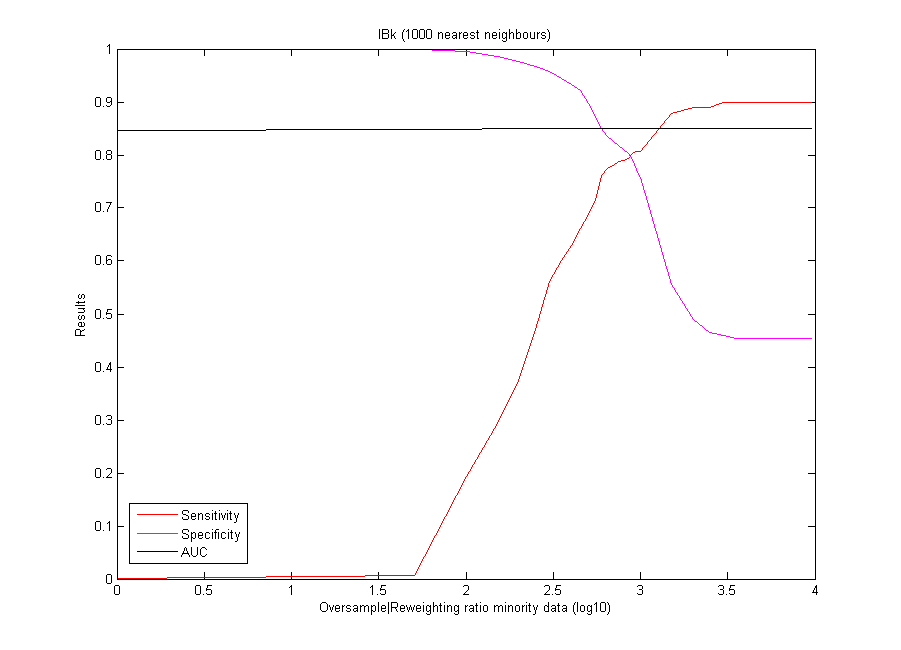
\includegraphics[scale=0.65]{img/bi_IBk-1000NN.png}
\caption{\textbf{Bagging with IBk} (1000NN) - Experiment results of Bagging for Imbalanced Datasets with IBk. This technique allows IBk to achieve a maximum AUC of 0.8507 at a misclassification cost of 9\,501. This classifier yields a sensitivity of 90.00\% and a specificity of 45.39\%. This is as well the highest obtained sensitivity.}
\end{figure}

\newpage
\begin{figure}[h]
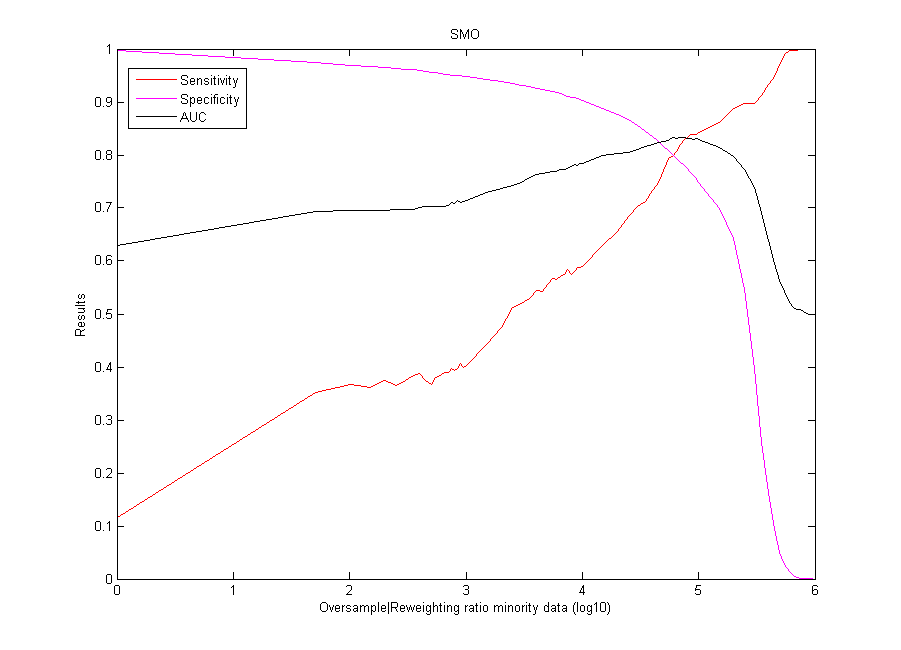
\includegraphics[scale=0.65]{img/bi_SMO.png}
\caption{\textbf{Bagging with SMO} (complexity parameter $c = 1$, linear exponent) - Experiment results of Bagging for Imbalanced Datasets with SMO. This technique allows SMO to achieve a maximum AUC of 0.8339 at a misclassification cost of 70\,001. This classifier yields a sensitivity of 81.94\% and a specificity of 78.65\%. A sensitivity of 91.29\% is achieved using a misclassification cost of 350\,001, and yields a specificity of 25.69\%. Finally, a maximum sensitivity of 100.00\% is obtained together with a specificity of 0.15\%.}
\end{figure}

\newpage
\subsection{Other Learning Techniques}\label{exp-other}

\subsubsection{REMED}
The following evaluations were performed by Prof. Luis Mena using the REMED learning algorithm. Some of the features needed to be preprocessed, as the REMED algorithm was initially developed to consider numeric or binary discrete attributes. For this reason, nominal attributes with three values \{0,1,2\} were converted such that (0= yes) is mapped to (0= present), and (1=no or 2=I don't know) is mapped to (1=absent).\\
Using a confidence level of p\textless{0.0001}, the three most statistically significant features were found to be \textit{Obs\_Different} (p=0), \textit{PE\_Something\_Wrong} (p=0) and \textit{Child\_seriously\_ill} (p=3,3307 e -16). These features are then used to generate independent classifiers:
\\ \\ \textbf{classifier 1} \\{\small \fbox{\parbox[b]{5in} {
(Obs\_different=0) =\textgreater{} serious\_without\_GE\_bronch=0 \\
=\textgreater{} serious\_without\_GE\_bronch=1}}}
\\ \\ \textbf{classifier 2} \\{\small \fbox{\parbox[b]{5in} {
(PE\_Something\_Wrong=0) =\textgreater{} serious\_without\_GE\_bronch=0 \\
=\textgreater{} serious\_without\_GE\_bronch=1}}}
\\ \\ \textbf{classifier 3} \\{\small \fbox{\parbox[b]{5in} {
(Child\_seriously\_ill=0) =\textgreater{} serious\_without\_GE\_bronch=0 \\
=\textgreater{} serious\_without\_GE\_bronch=1}}}
\\ \\ When the continuous attributes are analysed, the only attribute to be found statistically significant (confidence leel of 99\%) is the age. This allows to build two better classifiers combining both types of attributes:
\\ \\ \textbf{classifier 4} \\{\small \fbox{\parbox[b]{5in} {
(PE\_Something\_Wrong=0) and (Age\textless{}=3.32) =\textgreater{} serious\_without\_GE\_bronch=0 \\
=\textgreater{} serious\_without\_GE\_bronch=1}}}
\\ \\ \textbf{classifier 5} \\{\small \fbox{\parbox[b]{5in} {
(Child\_seriously\_ill=0) and (Age\textless{}=3.32) =\textgreater{} serious\_without\_GE\_bronch=0 \\
=\textgreater{} serious\_without\_GE\_bronch=1}}}

\newpage
The results for each classifier are showed in the following table, where the AUC was calculated with the conventional binormal method through PLOTROC.xls, available at \url{http://xray.bsd.uchicago.edu/krl/KRL_ROC/software_index.htm}


\begin{tabular}{l l l l l l l}
\cr
\hline
Classifier & Accuracy & Sensitivity & Specificity & AUC & GM & Ranker \\
\hline
1 & 96,4295 & 41,1765 & 96,8982 & 65,97 & 63,1662 & 64,57 \\
2 & 96,9998 & 55,8824 & 97,3493 & 71,18 & 73,7571 & 72,47 \\
3 & 92,3382 & 58,8235 & 92,6232 & 72,13 & 73,8134 & 72,97 \\
4 & 98,2147 & 41,1765 & 98,6997 & 65,97 & 63,7503 & 64,57 \\
5 & 96,2063 & 41,1765 & 96,6742 & 65,97 & 63,0928 & 72,47 \\
\hline
\cr
\end{tabular}

\paragraph*{Conclusion}Although REMED is developed to focus on the class imbalance problem, resulting classifiers are not satisfiable for practical purpose due to the low sensitivities. 

\newpage
\subsubsection{Thresholding Naive Bayes}
Cost-sensitivity analysis showed that the highest AUC (namely 0.9040) is obtained by a Naive Bayes classifier. For this reason, we analyse the effect of altering the class probability threshold for this classifier.
\begin{figure}[h]
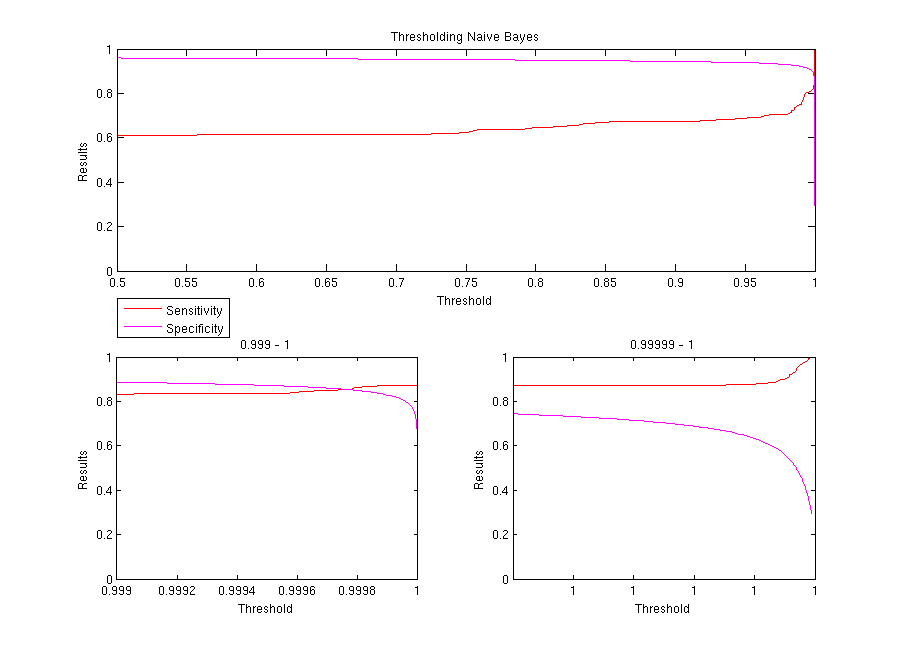
\includegraphics[scale=0.65]{img/thh_naivebayes.png}
\end{figure}

Results show that increasing the threshold can significantly affect the sensitivity. For example, when the threshold is altered from 50\% to 99.9999\%, a sensitivity of 90.3226\% and a specificity of 55.8177\%.


\newpage
\subsection{Summary}\label{exp-summary}
The following tables show an overview of the experiment results. For each experiment, the highest achieved AUC (and the the sample ratio to obtain this classifier) is displayed together with the highest obtained sensitivity (and the resulting specificity).

\begin{table}[h]
\centering  
\begin{tabular}{ l | c r | r r|}                                      
& \multicolumn{2}{c}{max AUC (sample ratio)} & \multicolumn{2}{c}{max sensitivity (specificity)} \\
\hline 
\multicolumn{5}{l}{\textbf{Cost-sensitivity}}\\
\hline
J48 (confidence factor 0.25) & 0.8536 & (13\,250) & 99.35\% & (0.67\%)\\
J48 (confidence factor 0.40) & 0.8478 & (18\,400) & 96.77\% & (6.21\%)\\
J48 (confidence factor 0.65) & 0.8431 & (19\,600) & 99.03\% & (1.32\%)\\
JRip (pruned) & 0.8431 & (466) & 99.03\% & (29.13\%)\\
JRip (unpruned) & 0.8473 & (33\,350) & 97.74\% & (43.00\%)\\
Naive Bayes (Laplace smoothing) & 0.9040 & (1) & 95.48\% & (26.95\%)\\
Naive Bayes (no smoothing) & 0.6653 & (1) & 65.16\% & (52.83\%)\\
IB3 & 0.5368 & (1) & 6.45\% & (99.59\%)\\
IB10 & 0.6044 & (1) & 20.65\% & (98.48\%)\\
IB50 & 0.7683 & (1) & 56.13\% & (95.71\%)\\
IB200 & 0.8182 & (1) & 69.68\% & (87.77\%)\\
IB1000 & 0.8539 & (601) & 90.00\% & (45.66\%)\\
IB2000 & 0.8644 & (5\,001) & 96.77\% & (1.48\%)\\
SMO & 0.8111 & (70\,250) & 84.52\% & (75.63\%)\\
CART (min 50 nodes/leaf) & - & - & 74.19\% & (91.19\%)\\
CART (min 100 nodes/leaf) & - & - & 77.42\% & (90.13\%)\\
CART (min 150 nodes/leaf) & - & - & 87.10\% & (64.67\%)\\
CART (min 200 nodes/leaf) & - & - & 80.65\% & (50.99\%)\\
\hline                          % inserts single-line
\end{tabular}
\label{tab:CostSens}
\caption{Summary of classifier performance (Cost-sensitivity)} % title name of the table
\end{table}

\paragraph{Cost-sensitivity} Results show that especially JRip and Naive Bayes (when estimates are smoothed by Laplace) are interesting classifiers when over-sampled (by means of cost-sensitivity). Decision tree classifiers such as J48 and CART on the other hand do not perform well when the minority class data is over-sampled. Although less pruning can increase the recognition of the minority class, it tends to decrease the recognition of the majority class. This observation confirms the discussion in section~\ref{causestheproblem} about the influence of class and feature noise on the recognition of outliers. A similar story happens with IBk. When the number of nearest neighbours is small (large), low recognition rates for the minority (majority) class are obtained. This observation is founded by the fact that nearest neighbours algorithms typically are sensitive to noise.

Finally, it is not clear how well SMO can perform in datasets with class imbalance. Because SMO is a very time-consuming algorithm, experiments were only performed using the most basic parameters and kernels. Hence, it is possible that the use of different kernels and/or complexity parameters can improve the performance.

\newpage
\paragraph{SMOTE} Synthetic sampling (such as SMOTE) was discussed as a another approach to sampling besides instance reweighting. Although SMOTE can decrease the risk of overfitting, experiment results are not very optimistic. In many tested classifiers, SMOTE obtains a worse performance than cost-sensitivity. Moreover, applying SMOTE with Naive Bayes learning decreases (rather than increases) the recognition rate of the minority class. The only classifier where SMOTE increases performance, is IBk. This is probably related to the fact that SMOTE performs local smoothing on the training set, which matches the inductive bias of $k$-nearest neighbours~\cite{joydeep07}. It should however be clear that the (minority) data is not always forming clusters of at least $k$ instances. When these assumptions are violated, SMOTE increases the level of noise. Given the pessimistic experiment results of SMOTE, we have reason to believe that these assumptions indeed do not hold in the KULeuven dataset.

\begin{table}[h]
\centering  
\begin{tabular}{ l | c r | r r|}                                      
& \multicolumn{2}{c}{max AUC (sample ratio)} & \multicolumn{2}{c}{max sensitivity (specificity)} \\
\hline
\multicolumn{5}{l}{\textbf{SMOTE}}\\
\hline
J48 (confidence factor 0.50) & 0.6750 & (151) & 13.87\% & (99.55\%)\\
JRip (unpruned) & 0.6096 & (801) & 23.23\% & (98.70\%)\\
Naive Bayes (Laplace smoothing) & 0.9040 & (1) & 64.52\% & (95.94\%)\\
IB1000 & 0.8616 & (1) & 74.52\% & (84.88\%)\\
SMO & 0.6145 & (51) & 23.55\% & (99.35\%)\\
\hline
\end{tabular}
\label{table:Performance02}
\caption{Summary of classifier performance (SMOTE)} % title name of the table
\end{table}

\paragraph{MetaCost} MetaCost mainly seems to have a positive effect on Naive Bayes classifiers. This is probably related to the fact that Naive Bayes learning strongly depends on the quality of the estimated prior estimates. Since MetaCost uses a bagging scheme to estimate the class probabilities, the quality of these estimates is improved. 

\begin{table}[h]
\centering  
\begin{tabular}{ l | c r | r r|}  
& \multicolumn{2}{c}{max AUC (sample ratio)} & \multicolumn{2}{c}{max sensitivity (specificity)} \\
\hline
\multicolumn{5}{l}{\textbf{MetaCost}}\\
\hline
J48 (confidence factor 0.40) & 0.7846 & (251) & 97.74\% & (0.00\%)\\
JRip (unpruned) & 0.6565 & (51) & 100.00\% & (0.00\%)\\
Naive Bayes (Laplace smoothing) & 0.9206 & (1) & 100.00\% & (12.54\%)\\
SMO & 0.6299 & (51) & 26.77\% & (99.22\%)\\
\hline
\end{tabular}
\label{table:Performance02}
\caption{Summary of classifier performance (MetaCost)} % title name of the table
\end{table}

\paragraph{Bagging for Imbalanced Datasets} Bagging for Imbalanced Datasets seems to have a positive influence on the performance of all classifiers. Because bagging reduces the variance, it helps to avoid overfitting (and therefore to increase the recognition rate of the minority class).

\begin{table}[h]
\centering  
\begin{tabular}{ l | c r | r r|}  
& \multicolumn{2}{c}{max AUC (sample ratio)} & \multicolumn{2}{c}{max sensitivity (specificity)} \\
\hline
\multicolumn{5}{l}{\textbf{Bagging for Imbalanced Datasets}}\\
\hline
J48 (confidence factor 0.40) & 0.8783 & (6500) & 100.00\% & (0.00\%)\\
JRip (unpruned) & 0.8976 & (7001) & 98.06\% & (44.56\%)\\
Naive Bayes (Laplace smoothing) & 0.9180 & (1) & 93.87\% & (27.76\%)\\
IB1000 & 0.8507 & (9501) & 90.00\% & (46.01\%)\\
SMO & 0.8339 & (70001) & 100.00\% & (0.15\%)\\
\hline
\end{tabular}
\label{table:Performance02}
\caption{Summary of classifier performance (Bagging for Imbalanced Datasets)} % title name of the table
\end{table}

\newpage
Finally, altering probability thresholds seems an interesting approach to improve classification in datasets with class imbalance, especially when applied to a Naive Bayes classifier. In general, altering the probability thresholds allows a good sensitivity-specificity tradeoff when applied to classifiers with a high AUC.

\begin{table}[h]
\centering  
\begin{tabular}{ l | c r | r r|}  
& \multicolumn{2}{c}{max AUC (sample ratio)} & \multicolumn{2}{c}{max sensitivity (specificity)} \\
\hline
\multicolumn{5}{l}{\textbf{Other}}\\
\hline
REMED & 0.7213 & - & 58.82\% & (92.62\%)\\
Naive Bayes (Thresholding) & 0.9040 & (1) & 99.68\% & (33.16\%)\\
\hline                          % inserts single-line
\end{tabular}
\label{table:Performance02}
\caption{Summary of classifier performance (Other)} % title name of the table
\end{table}



%-------------------------------------------------------------------------------------------------------------------
% RNB-FVB
%-------------------------------------------------------------------------------------------------------------------
\newpage
\section{Experiment results of Naive Bayes Sampling}\label{exp-rnb}
In this section, we investigate the performance of Naive Bayes Sampling by applying different sampling ratios, as introduced in chapter~\ref{newapproach}. The number of Naive Bayes classifiers in each ensemble is restricted to 10. 
We evaluate the classifiers by applying stratified 10-fold cross-validation (which is repeated over 10 randomized runs), and measure the AUC, sensitivity and specificity. Afterwards, we compare these results to the ones obtained by combining Naive Bayes learning with Cost-Sensitivity (see section~\ref{cost-sensitivity}), MetaCost and Bagging for Imbalanced Datasets (see section~\ref{classif-ensembles}).

\newpage
\subsection{Ill Children (KULeuven)}
\begin{figure}[h]
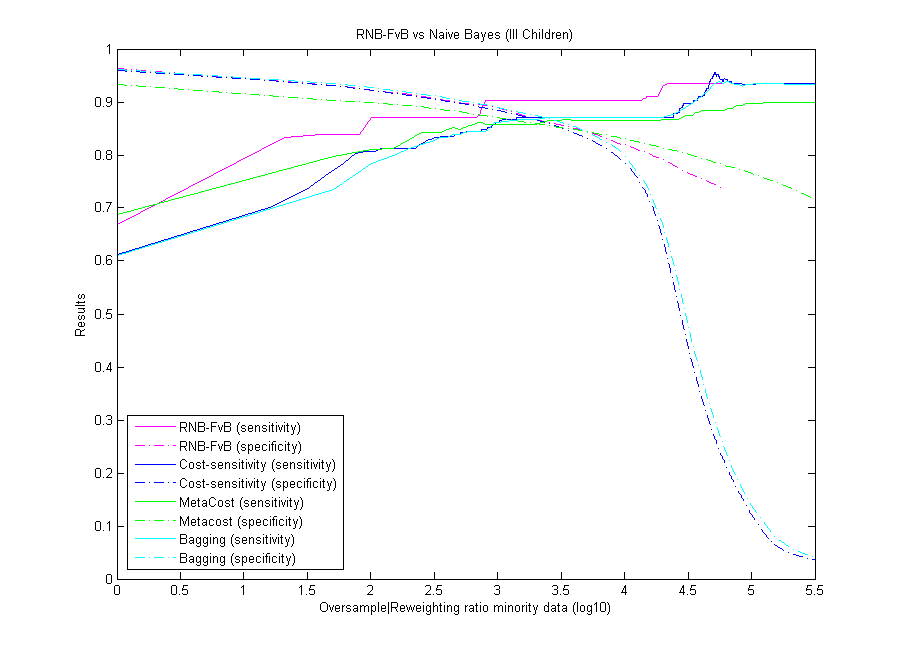
\includegraphics[scale=0.65]{img/RNB-FvB-illchildren.png}
\caption{Experiment results of Naive Bayes Sampling on \textbf{Ill Children}}
\end{figure}
 
\begin{table}[h]
\centering  
\begin{tabular}{ l | c r | r r|}                                      
& \multicolumn{2}{c}{max AUC (sample ratio)} & \multicolumn{2}{c}{max sensitivity (specificity)} \\
\hline 
Naive Bayes Sampling & 0.9479 & (x\,60\,000) & 93.55\% & (78.61\%)\\
Cost-sensitivity & 0.9040 & (x\,1) & 95.48\% & (26.95\%)\\
MetaCost & 0.9206 & (x\,1) & 100.00\% & (12.54\%)\\
Bagging & 0.9190 & (x\,1) & 93.87\% & (27.76\%)\\
\hline                          % inserts single-line
\end{tabular}
\label{tab:PPer}
\caption{Overview Results Naive Bayes Sampling for Ill Children} % title name of the table
\end{table}
 

\newpage
\subsection{Breast-Cancer (UCI)}
\begin{figure}[h]
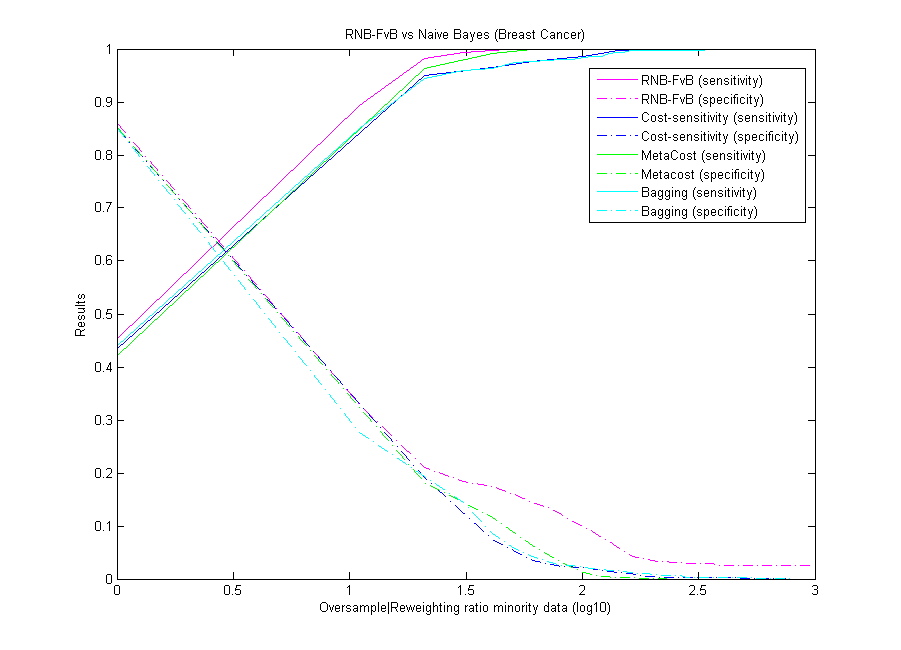
\includegraphics[scale=0.65]{img/RNB-FvB-breastcancer.png}
\caption{Experiment results of Naive Bayes Sampling on \textbf{Breast Cancer}}
\end{figure}

\begin{table}[h]
\centering  
\begin{tabular}{ l | c r | r r|}                                      
& \multicolumn{2}{c}{max AUC (sample ratio)} & \multicolumn{2}{c}{max sensitivity (specificity)} \\
\hline 
Naive Bayes Sampling & 0.7450 & (x\,271) & 100.00\% & (15.92\%)\\
Cost-sensitivity & 0.6981 & (x\,1) & 100.00\% & (0.30\%)\\
MetaCost & 0.7187 & (x\,41) & 100.00\% & (3.03\%)\\
Bagging & 0.6995 & (x\,1) & 100.00\% & (0.00\%)\\
\hline                          % inserts single-line
\end{tabular}
\label{tab:PPer}
\caption{Overview Results Naive Bayes Sampling for Breast Cancer} % title name of the table
\end{table}


\newpage
\subsection{Hepatitis (UCI)}
\begin{figure}[h]
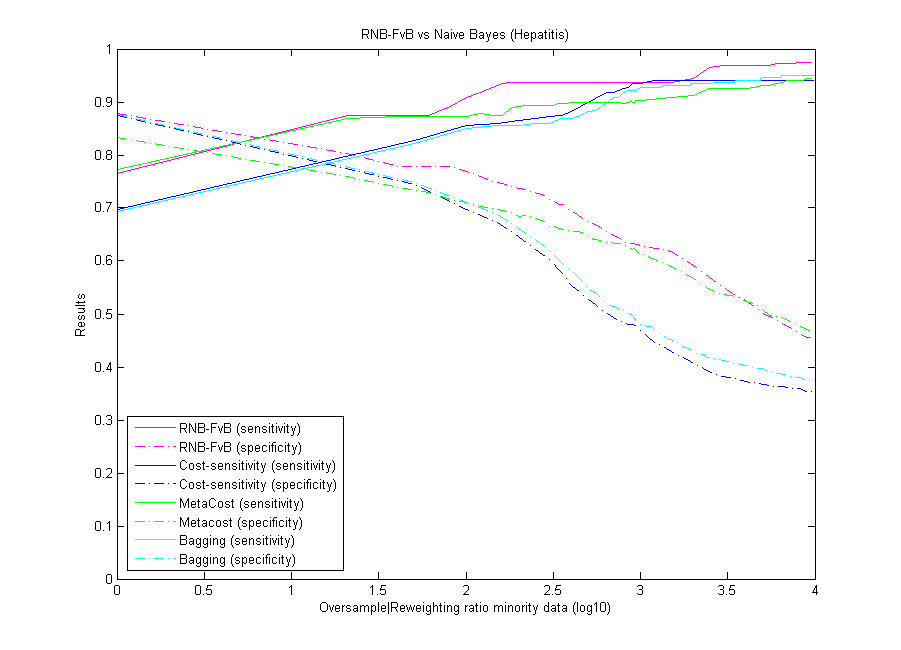
\includegraphics[scale=0.65]{img/RNB-FvB-hepatitis.png}
\caption{Experiment results of Naive Bayes Sampling on \textbf{Hepatitis}}
\end{figure}

\begin{table}[h]
\centering  
\begin{tabular}{ l | c r | r r|}                                      
& \multicolumn{2}{c}{max AUC (sample ratio)} & \multicolumn{2}{c}{max sensitivity (specificity)} \\
\hline 
Naive Bayes Sampling & 0.9101 & (x\,7\,500) & 97.50\% & (46.42\%)\\
Cost-sensitivity & 0.8639 & (x\,51) & 94.06\% & (44.72\%)\\
MetaCost & 0.8710 & (x\,21) & 94.37\% & (47.07\%)\\
Bagging & 0.8746 & (x\,51) & 95.00\% & (38.86\%)\\
\hline                          % inserts single-line
\end{tabular}
\label{tab:PPer}
\caption{Overview Results Naive Bayes Sampling for Hepatitis} % title name of the table
\end{table}

\newpage
\subsection{Sick (UCI)}
\begin{figure}[h]
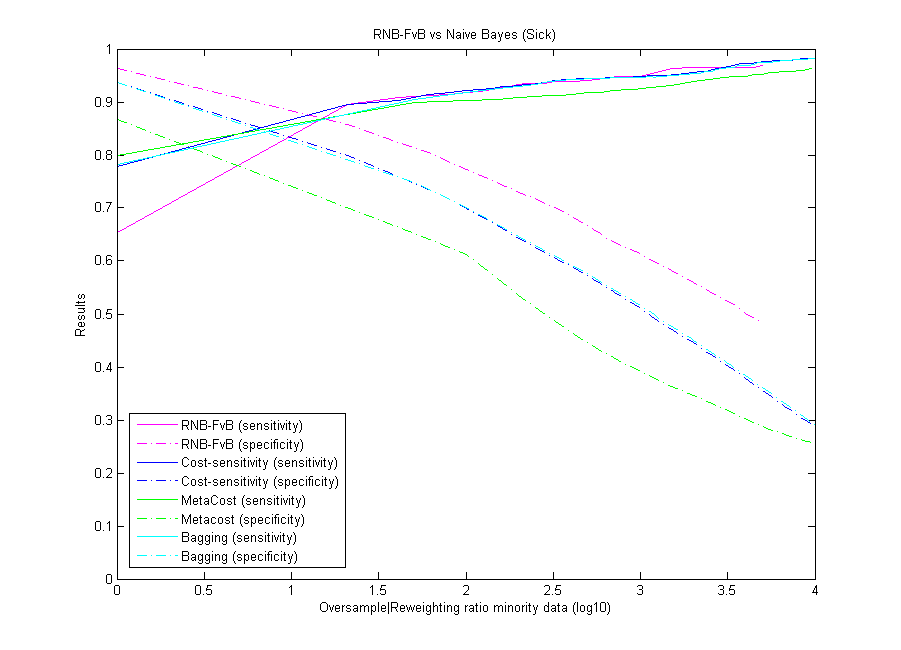
\includegraphics[scale=0.65]{img/RNB-FvB-sick.png}
\caption{Experiment results of Naive Bayes Sampling on \textbf{Sick}}
\end{figure}

\begin{table}[h]
\centering  
\begin{tabular}{ l | c r | r r|}                                      
& \multicolumn{2}{c}{max AUC (sample ratio)} & \multicolumn{2}{c}{max sensitivity (specificity)} \\
\hline 
Naive Bayes Sampling & 0.9322 & (x\,1) & 96.97\% & (48.18\%)\\
Cost-sensitivity & 0.9253 & (x\,1) & 98.23\% & (29.74\%)\\
MetaCost & 0.8898 & (x\,1) & 96.23\% & (25.73\%)\\
Bagging & 0.9269 & (x\,1) & 98.18\% & (29.32\%)\\
\hline                          % inserts single-line
\end{tabular}
\label{tab:PPer}
\caption{Overview Results Naive Bayes Sampling for Sick} % title name of the table
\end{table}

\newpage
\subsection{Liver disorders (UCI)}
\begin{figure}[h]
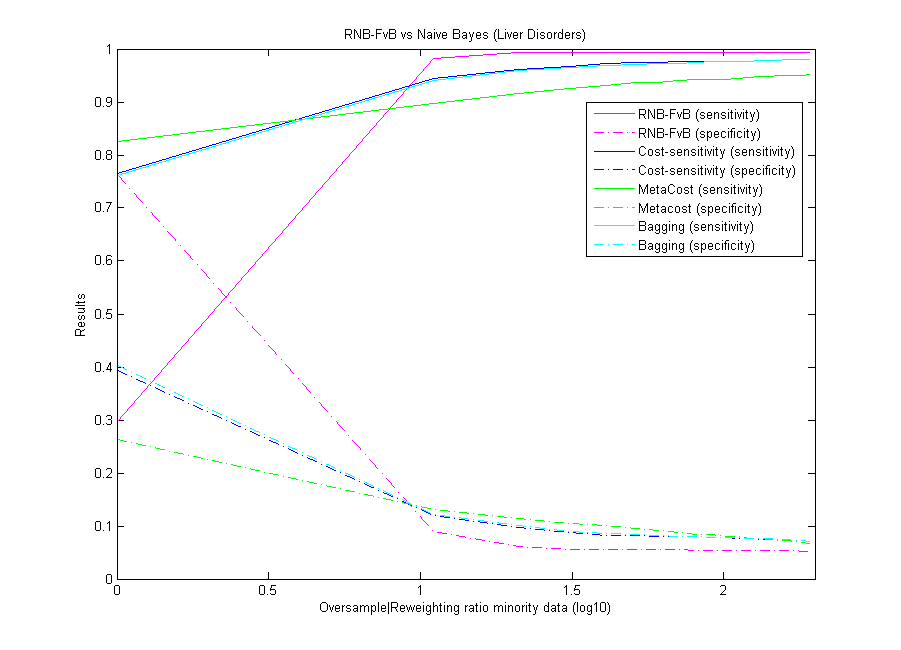
\includegraphics[scale=0.65]{img/RNB-FvB-liverdisorder.png}
\caption{Experiment results of Naive Bayes Sampling on \textbf{Liver Disorders}}
\end{figure}

\begin{table}[h]
\centering  
\begin{tabular}{ l | c r | r r|}                                      
& \multicolumn{2}{c}{max AUC (sample ratio)} & \multicolumn{2}{c}{max sensitivity (specificity)} \\
\hline 
Naive Bayes Sampling & 0.5744 & (x\,11) & 99.31\% & (6.05\%)\\
Cost-senstivity & 0.6331 & (x\,171) & 97.93\% & (7.25\%)\\
MetaCost & 0.5804 & (x\,11) & 95.10\% & (6.75\%)\\
Bagging & 0.6289 & (x\,161) & 97.93\% & (7.40\%)\\
\hline                 
\end{tabular}
\label{tab:PPer}
\caption{Overview Results Naive Bayes Sampling for Liver Disorders} 
\end{table}





